\documentclass[letterpaper,journal]{IEEEtran}
\usepackage{amsmath,amsfonts}
\usepackage{algorithmic}
\usepackage{array}
\usepackage[caption=false,font=normalsize,labelfont=sf,textfont=sf]{subfig}
\usepackage{textcomp}
\usepackage{stfloats}
\usepackage{url}
\usepackage{verbatim}
\usepackage{graphicx}
\hyphenation{op-tical net-works semi-conduc-tor IEEE-Xplore}
\def\BibTeX{{\rm B\kern-.05em{\sc i\kern-.025em b}\kern-.08em
    T\kern-.1667em\lower.7ex\hbox{E}\kern-.125emX}}
\usepackage{balance}
\usepackage{newtxtext}
\usepackage{newtxmath}
\usepackage{float}
\usepackage{tabularx}
\usepackage{makecell}
\usepackage{lipsum}
\usepackage{xcolor}
\usepackage{placeins}
\usepackage{datetime}
\usepackage{enumitem}
\usepackage[switch]{lineno}
\newdateformat{monthyeardate}{\monthname[\THEMONTH] \THEYEAR}

\linenumbers

% correct bad hyphenation here
\hyphenation{op-tical net-works semi-conduc-tor}


\begin{document}
%
% paper title
\title{The Extended Polarimetric Slope Sensing Technique}

\author{Nathan~J.~M.~Laxague,~\IEEEmembership{Member,~IEEE,}
        Z.~G\"oksu~Duvarc\i,\\
        Lindsay~Hogan, Junzhe~Liu,
        Christopher~Bouillon, and Christopher~J.~Zappa% <-this % stops a space
\thanks{N. J. M. Laxague is with the Department
of Mechanical Engineering and Center for Ocean Engineering, University of New Hampshire, Durham, NH, USA e-mail: Nathan.Laxague@unh.edu.}% <-this % stops a space
\thanks{Z. G. Duvarc\i~ is with the Center for Ocean Engineering, University of New Hampshire; L. Hogan and C. J. Zappa are with Lamont-Doherty Earth Observatory of Columbia University; C. Bouillon is with Institut des Sciences de la Mer, Université du Québec à Rimouski, Rimouski, QC, Canada.}% <-this % stops a space
\thanks{Manuscript received XXX; revised YYY.}}

% The paper headers
\markboth{IEEE Journal of Selected Topics in Applied Earth Observations and Remote Sensing,~Vol.~XX, No.~YY, \monthyeardate\today}%
{Laxague \MakeLowercase{\textit{et al.}}: Subpixel Variability and Polarimetric Slope Sensing}

% make the title area
\maketitle

% As a general rule, do not put math, special symbols or citations
% in the abstract or keywords.
\begin{abstract}
TEXT

\end{abstract}

% Note that keywords are not normally used for peerreview papers.
\begin{IEEEkeywords}
Polarimetry, gravity-capillary waves, wave slope sensing, polarimetric slope sensing, division of focal plane
\end{IEEEkeywords}

% For peerreview papers, this IEEEtran command inserts a page break and
% creates the second title. It will be ignored for other modes.
\IEEEpeerreviewmaketitle

\textbf{Outline}

\begin{itemize}
    \item PSS is useful, but there are two main issues to address:
    \begin{enumerate}
        \item Unknown impact of ambient illumination conditions on surface wave measurements.
        \begin{enumerate}
        \item impact of polarized incident light
        \item impact of upwelling light
        \item this makes the DoLP-$\theta$ relationship different for each measurement
    \end{enumerate}
        \item Previous applications of PSS have been scale-limited to target short waves at the expense of long waves
        \begin{enumerate}
            \item Integrating a robust long wave sensing component into the PSS framework would significantly expand the technique's usefulness
        \end{enumerate}
        \item \textbf{We need to address these concerns without adding any more cameras: all we get is one imager that stays looking at the sea surface.}
    \end{enumerate}
    \item Let's address the first challenge first. What are our options?
    \begin{enumerate}
        \item laboratory-based gain to DoLP
        \item measurement of upwelling radiance and downwelling polarization state
        \item direct measurement of DoLP-$\theta$ relationship with wide format lens
        \item absent all of that-- an \lq\lq empirical" gain; \textbf{this is what we're going with here}
    \end{enumerate}
    \item The second challenge:
    \begin{enumerate}
        \item transfer function: inferring the water surface elevation time series from the two-component surface slope time series
        \item integrate the slope fields to obtain small-scale roughness variation
        \item inferring frequency-directional spectrum from virtual wave gauge array (MEM/EMEP and E-WDM)
    \end{enumerate}
    \item Our Results
    \begin{enumerate}
        \item timeseries comparison (lidar)
        \item spectra comparison (lidar)
        \item significant wave height comparison (lidar)
        \item wave direction and spreading comparison (ADCP)
        \item slope statistics with wind speed (mss, PDFs, skewness/kurtosis)
        \item wave spectra with wind speed
    \end{enumerate}
    \item Going forward: adding more imagers for \emph{in situ} determination of ambient illumination conditions
    \begin{enumerate}
        \item Wide format surface imager, for direct measurement of DoLP-$\theta$ relationship. Need to consider effects of light rays entering FPA obliquely \cite{pistellato_geometric_2024}.
    \end{enumerate}
\end{itemize}

\section{Background}
\label{sec:intro}
\IEEEPARstart{F}{irst} sentence.\\

Some relevant papers on the topic: \cite{Zappa2008}, \cite{laxague_effects_2025}.

\section{Methodology}
\label{sec:methodology}

\section{Results}
\label{sec:results}

\section{Discussion}
\label{sec:discussion}

% use section* for acknowledgment
\section*{Acknowledgment}

The ASIT2019 field observations were made with the assistance of Steve Faluotico, Jay Sisson, the crew of the \textit{R/V Tioga}, and Carson Witte \& Suki Wong.\\

% Collection of field data from \textit{R/P FLIP} was supported by ONR (grants N00014-06-1-0372 and
% N00014-11-1-0168).
Collection of field data from ASIT was supported by NSF (Award Number 1756839), ONR (Award Number N00014-22-1-2183), and NASA (Award Number 80NSSC19K1397). Analysis of the ASIT2019 dataset was supported by NSF award 20-49578 (NJML \& CJZ). NJML was also supported by NSF award 23-40712.\\

The full suite of codes which contain our implementation of Polarimetric Slope Sensing (PSS) for DoFP polarimeters are available at \url{https://github.com/unh-cassll/polarimetric-slope-sensing}.

Finally-- all of the codes used to produce the graphics shown in this document are available at \url{https://github.com/unh-cassll/E-PSS}.

% references section

\newpage

\bibliographystyle{IEEEtran}
\bibliography{references}

\newpage

\begin{IEEEbiography}[{
\includegraphics[width=1in,height=1.25in,clip,keepaspectratio]{_figures/headshot_laxague.jpg}}]{Nathan J. M. Laxague}
(M '16) earned a Bachelor of Science in Physics in 2011 from the University of Miami, Coral Gables, FL USA. He received his Ph.D. in Applied Marine Physics from the Rosenstiel School of Marine and Atmospheric Sciences at the University of Miami in 2016. He was a postdoctoral research scientist at Lamont-Doherty Earth Observatory of Columbia University, in Palisades, NY, USA from 2017-2020. Since 2020, he has been an Assistant Professor of Ocean Engineering in the Department of Mechanical Engineering at the University of New Hampshire in Durham, NH, USA.
\end{IEEEbiography}

\begin{IEEEbiography}
[{
\includegraphics[width=1in,height=1.25in,clip,keepaspectratio]{_figures/headshot_duvarci.jpg}}]{Z. G\"oksu Duvarc\i}
earned a Bachelor of Science in Chemical Engineering with a Minor in Mechanical Engineering in 2022 from Bo\v gazi\c ci University in Istanbul, Turkey. She is currently a Ph.D. student in Ocean Engineering at the University of New Hampshire in Durham, NH, USA.
\end{IEEEbiography}

\begin{IEEEbiography}[{
\includegraphics[width=1in,height=1.25in,clip,keepaspectratio]{_figures/headshot_hogan.jpg}}]{Lindsay Hogan}
(M '24) earned a Bachelor of Science in Geology and Geophysics in 2020 from Yale University, New Haven, CT, USA. She received a Masters by Research in Climate and Atmospheric Science in 2021 from the University of Leeds, Leeds, UK. Lindsay earned a Master of Arts in Earth and Environmental Sciences from Columbia University in New York, NY, USA in 2023 and is currently a Ph.D. Candidate in Earth and Environmental Sciences at Columbia University and Lamont-Doherty Earth Observatory in Palisades, NY, USA.
\end{IEEEbiography}

\begin{IEEEbiography}[{
\includegraphics[width=1in,height=1.25in,clip,keepaspectratio]{_figures/headshot_anderson.jpg}}]{Junzhe Liu}
% earned a Bachelor of Science in Mechanical Engineering in 1987 from Lafayette College, Easton, PA, USA. He received his Ph.D. in Applied Ocean Sciences in 1992 from Scripps Institution of Oceanography, U.C. San Diego, CA, USA and completed his Postdoctoral Scholar Award at the Woods Hole Oceanographic Institution in 1994 in Woods Hole, MA, USA. He is currently a Fellow at Aret\'{e} located in Niwot, CO, USA.
\end{IEEEbiography}

\begin{IEEEbiography}[{
\includegraphics[width=1in,height=1.25in,clip,keepaspectratio]{_figures/headshot_anderson.jpg}}]{Christopher Bouillon}
% earned a Bachelor of Science in Mechanical Engineering in 1987 from Lafayette College, Easton, PA, USA. He received his Ph.D. in Applied Ocean Sciences in 1992 from Scripps Institution of Oceanography, U.C. San Diego, CA, USA and completed his Postdoctoral Scholar Award at the Woods Hole Oceanographic Institution in 1994 in Woods Hole, MA, USA. He is currently a Fellow at Aret\'{e} located in Niwot, CO, USA.
\end{IEEEbiography}

\begin{IEEEbiography}[{
\includegraphics[width=1in,height=1.25in,clip,keepaspectratio]{_figures/headshot_zappa.jpg}}]{Christopher J. Zappa}
(M '03) earned a Bachelor of Science in Mechanical Engineering in 1992 from Columbia University, NY, NY, USA.  He received his Masters in Engineering in 1994 and his Ph.D. in Applied Ocean Physics in 1999 from the University of Washington, Seattle, WA, USA, and completed his Postdoctoral Scholar Award at the Woods Hole Oceanographic Institution in 2003 in Woods Hole, MA, USA. He is currently a Lamont Research Professor in and the Associate Director of Ocean and Climate Physics at Lamont-Doherty Earth Observatory in Palisades, NY, USA, and a Lecturer in the Department of Earth and Environmental Sciences in NY, NY, USA, both at Columbia University.
\end{IEEEbiography}

\end{document}

% FROM LAST TGRS PAPER

%Polarimetric slope sensing is a powerful and flexible technique for remote measurement of the air-sea interface. However, the effects of subpixel slope variability on the measurement itself are poorly described. We identify two principal areas of concern: (1) the process of computing wave slope from polarized light intensity is nonlinear, so variability may introduce net-nonzero biases; (2) novel Division of Focal Plane detectors make spatially non-collocated polarization measurements. Through interpretation of field observational data and the output of a numerical light reflection model, we find that both effects negatively impact wave slope field reconstruction, particularly for pixel sizes greater than 1 cm. These results are important for future application of the technique from airborne platforms.

% \IEEEPARstart{S}{hort} ocean waves are critical mediators of physical interactions between the earth's atmosphere and oceans. The intimate connection between surface wave state and air-sea interaction has been exploited to a great degree by electromagnetic remote sensing techniques. However, each particular technique (e.g., microwave SAR, X-band marine radar, HF radar) offers information along a specific scale and direction, necessitating the development of techniques which are able to illuminate a fuller set of details in the surface wave field. Characterization of surface waves with lengthscales less than 1 m have been the highest priority (due to their crucial role in mediating air-sea fluxes \cite{Makin1995,Kudryavtsev2002,Hwang2005}) and the source of the greatest vexation (due largely to the contamination of frequency-based analysis by mean currents and wave orbital advection). Imaging techniques such as stereophotogrammetry \cite{Banner1989,Benetazzo2006,Bergamasco2021} allow one to reconstruct the instantaneous sea surface over spatial scales ranging from decameters to decimeters. Amplitudes are at or below the displacement accuracy for photogrammetry for waves which are partially or predominantly restored to equilibrium by capillarity (wavelength $\lambda\lessapprox$6 cm \cite{Laxague2015}). However, the slope signal at those spatial scales is suitably large to enable reliable sensing of the surface slope field; this was first done in laboratory wind-wave tanks \cite{Jahne1990,Zhang1994,Zhang1995}, but developments in the 1990s enabled field observations of wave slope spectra \cite{Hara1994,Bock1995a}. The development of polarimetric slope sensing (PSS) \cite{Zappa2008} enabled non-contact monocular passive sensing of surface waves with lengths down to millimeters and periods down to less than one tenth of a second.

% However, polarimetric slope sensing remained a somewhat niche technique, with wide adoption hampered by the prohibitively expensive/custom equipment required to make precise polarization measurements with sufficiently small ($\approx$1 ms) integration times \cite{Zappa2012}. However, Division of Focal Plane (DoFP) polarimetric sensors---e.g., the increasingly-popular Sony Polarsens CMOS IMX253MZR---host integrated on-detector micropolarizer grid arrays, allowing for synchronous polarization sensing with low integration times. The wide commercial availability and low cost (10-100$\times$ less than previous generations) of the cameras which contain these detectors has brought a renewed interest in PSS. This renewed interest justifies the investigation of two concerns-- one (C1) long-standing with PSS and one (C2) newly presented by the DoFP detector design:\\
% \emph{C1: Spatial averaging of polarization state is not necessarily equivalent to spatial averaging of surface orientation.}
% \begin{itemize}
%     \item As the spatial footprint of an individual pixel increases, to what degree does sub-pixel variability in slope impact calculations of sea surface slope (Figure \ref{fig:MelvilleFedorov2015_surface_DoLP_example})?
% \end{itemize}
% \emph{C2: Polarization intensity measurements made by DoFP polarimeters are spatially sparse (non-collocated).}
% \begin{itemize}
%     \item Does this spatial sparseness inherent to DoFP polarimeters create aberrations in the computed slope field?
% \end{itemize}

% \vspace{-10pt}

% \begin{figure}[!ht]
% \centering
% 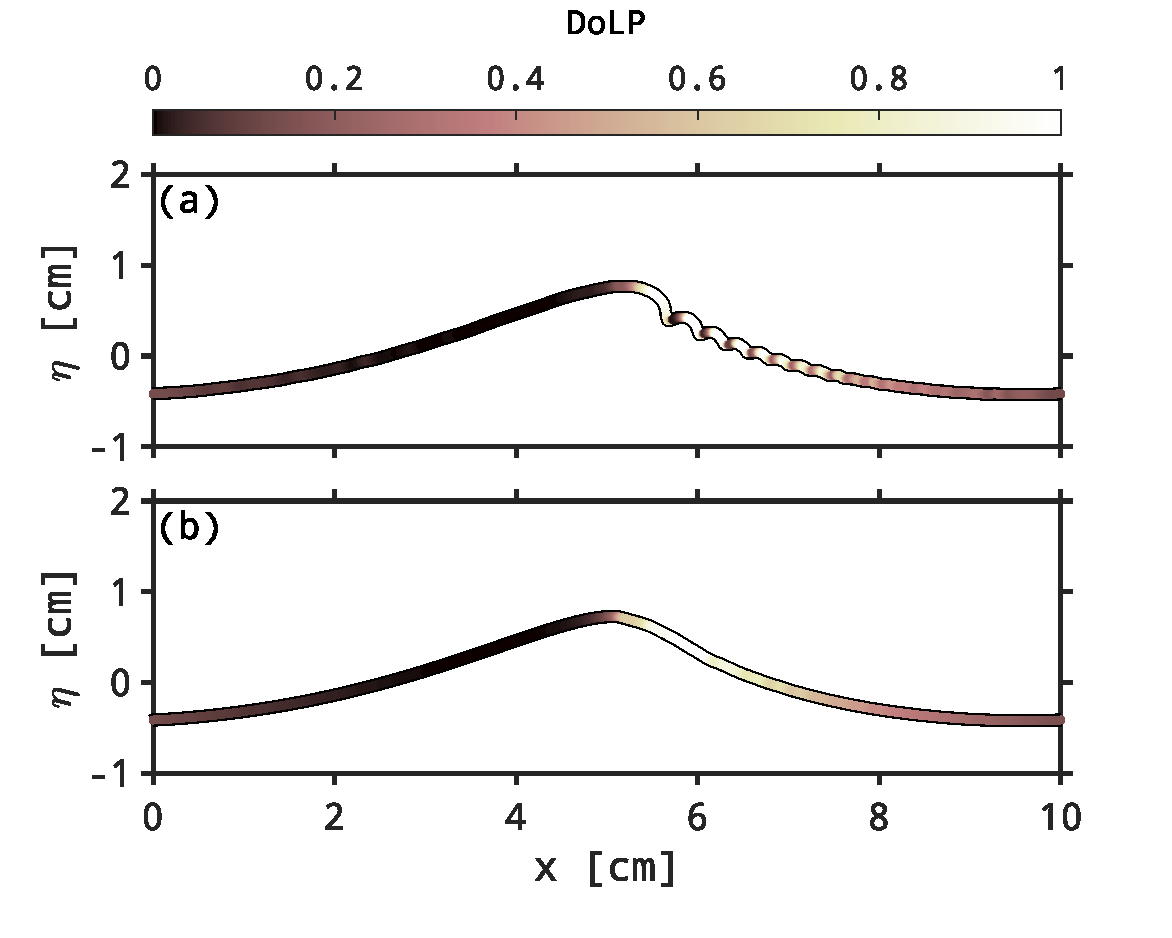
\includegraphics[width=0.5\textwidth]{_figures/MelvilleFedorov2015_surface_DoLP_example.pdf}
% \caption{Degree of linear polarization (DoLP) of modeled light \cite{mobley_polarized_2015} reflected from the surface of a simulated \cite{Melville2015} gravity-capillary wave: (a) full (0.01 cm) resolution, (b) wave subjected to 1-cm moving smoothing filter.}
% \label{fig:MelvilleFedorov2015_surface_DoLP_example}
% \end{figure}

% The work of applying the fundamental developments of Stokes and Mueller to the problem of remote sensing of ocean waves stretches back approximately forty years from the present day \cite{wolff_surface_1988,kattawar_stokes_1989}. Zappa \emph{et al.} \cite{Zappa2008} provided a self-contained, practical description of the steps required to infer water surface slope fields from observations of polarization state. Given measurement of the intensity of linearly polarized (0$^{\circ}$, 45$^{\circ}$, 90$^{\circ}$, \& 135$^{\circ}$) light across a spatial array, we may compute the normalized Stokes parameters $\Tilde{S}_{1}$ and $\Tilde{S}_{2}$:
% \begin{align}
%     %S_0 &= \frac{1}{2}\Big[I_0+I_{45}+I_{90}+I_{135}\Big]
%     \label{eq:Stokes1}
%     \Tilde{S}_{1} &= \frac{I_{0}-I_{90}}{I_{0}+I_{90}}\\
%     \label{eq:Stokes2}
%     \Tilde{S}_{2} &= \frac{I_{45}-I_{135}}{I_{45}+I_{135}}
% \end{align}

% Measurement of the Stokes parameters allow one to compute the polarization orientation ($\varphi$) and degree of linear polarization (DoLP) at each at each point in the imager field of view.
% \begin{align}
%     \label{eq:DoLP_stokes}
%     \mathrm{DoLP} &= \sqrt{\Tilde{S}_{1}^2+\Tilde{S}_{2}^2}\\
%     \label{eq:phi_stokes}
%     \varphi &= \frac{1}{2}\tan^{-1}\Big(\frac{\Tilde{S}_{2}}{\Tilde{S}_{1}}\Big)
% \end{align}

% DoLP itself varies with the specular reflection angle of incidence ($\theta$) and the real index of refraction ($n$). If we assume that sky-leaving radiance is unpolarized and upwelling (surface-leaving) radiance is negligible, we may simplify the Mueller calculus \cite{kattawar_stokes_1989,Zappa2008} and represent DoLP in terms of incidence angle and index of refraction:
% \begin{align}
%     \label{eq:DoLP_theta}
%     \mathrm{DoLP}(\theta,n) = \frac{2 \sin^2(\theta) \cos(\theta) \sqrt{n^2 - \sin^2(\theta)}}{n^2-\sin^2(\theta)-n^2\sin^2(\theta) +2 \sin^4(\theta)}
% \end{align}

% Calculation of $\varphi$ may be done directly through equation \ref{eq:phi_stokes}. However, inversion of equation \ref{eq:DoLP_theta} to obtain $\theta$ given DoLP (and an assumed/measured $n$) is non-trivial; a nonlinear solver would be prohibitively expensive to run for each pixel (order one million) in the frame, while use of a least-squares polynomial fit would risk the introduction of systematic bias at extreme low and high angles of incidence.

% \begin{figure*}[!hb]
% \centering
% 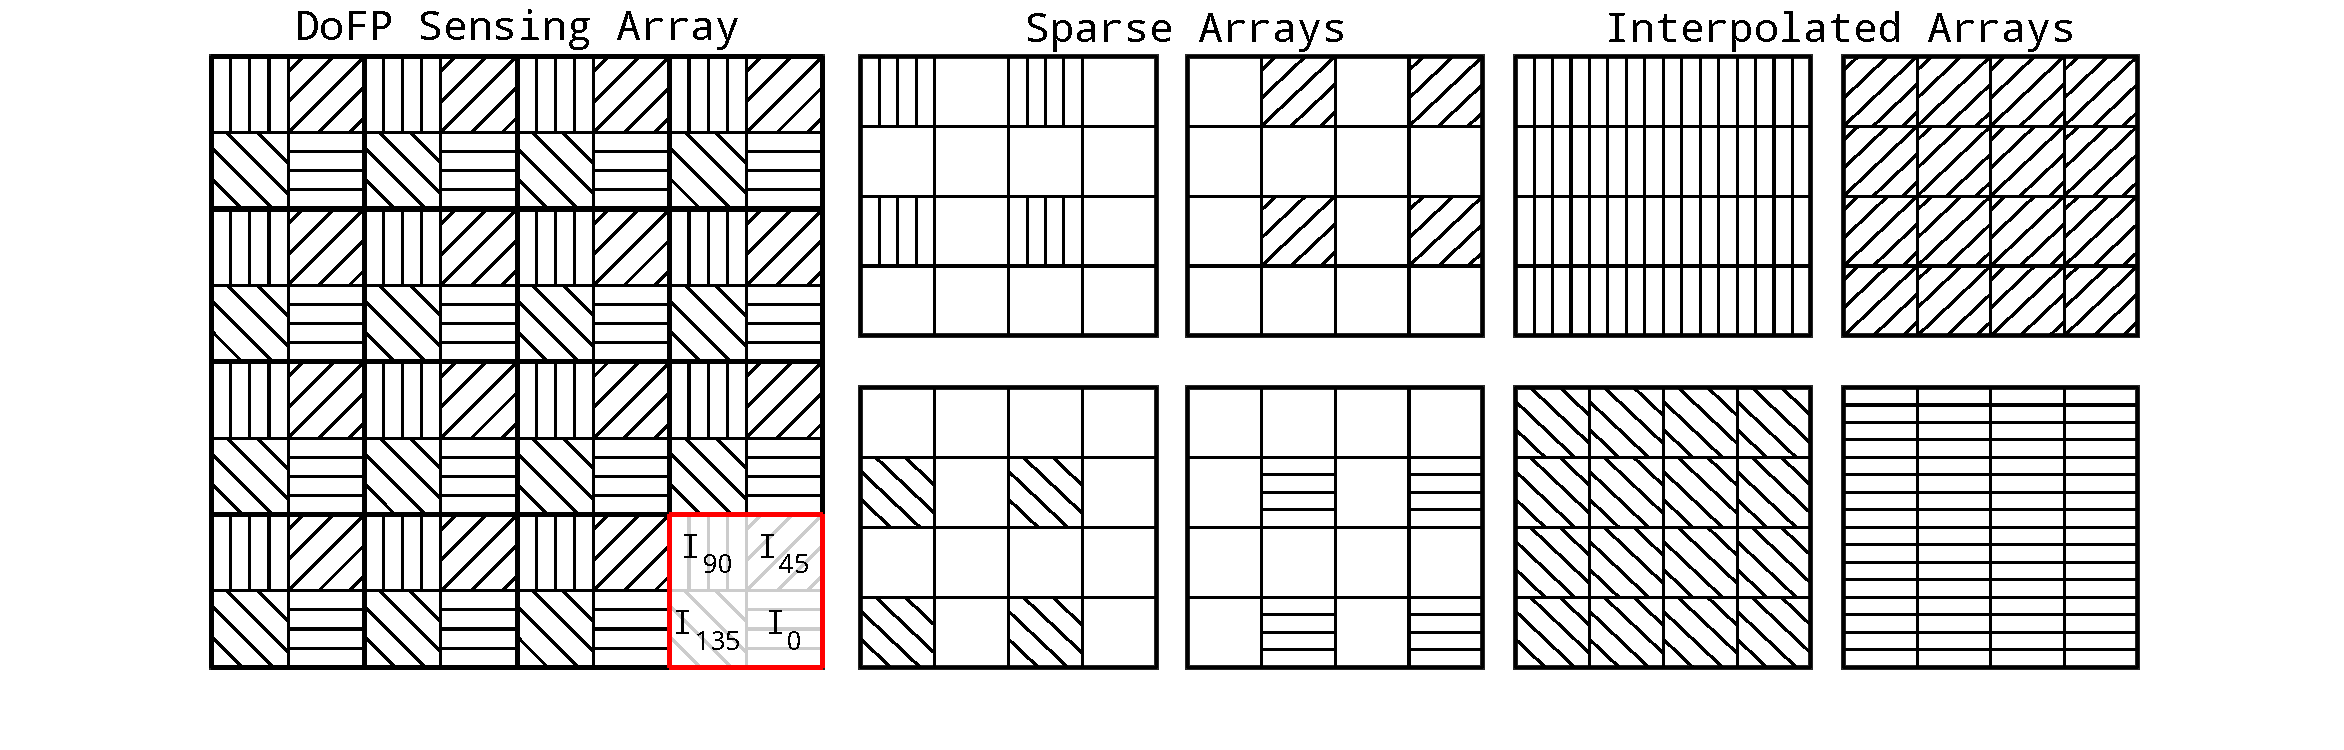
\includegraphics[width=\textwidth]{_figures/DoFP_superpixel_and_interpolation.pdf}
% \caption{Left: Division of Focal Plane (DoFP) array, with line segments indicating orientation of on-pixel micropolarizers; red boxed region represents a single \lq superpixel' containing one of each micropolarizer. Center: sparse arrays obtained in post-processing, each containing only a single component (e.g., $I_{45}$) of polarized light. Right: arrays produced via bilinear interpolation of sparse arrays, yielding a value of the linear polarization state [$I_{0}$,$I_{45}$,$I_{90}$,$I_{135}$] at each point.}
% \label{fig:DoFP_superpixel_and_interpolation}
% \end{figure*}

% Our chosen mode of operation has been to use a \lq\lq lookup table" of sorts, wherein $\theta$ is defined at $\lessapprox$0.1$^{\circ}$ resolution and the corresponding DoLP is computed. These values of $\theta$ are then mapped via cubic interpolation onto an array of 10$^4$ evenly-spaced levels in DoLP ranging from 0 to 1 and then saved to file for use in all future observations. After arrays of Stokes parameters have been obtained from observed polarized light intensities (equations \ref{eq:Stokes1}\&\ref{eq:Stokes2}) and DoLP has been computed (equation \ref{eq:DoLP_stokes}), the DoLP is rounded to the nearest 1$\times$10$^{-4}$ and then multiplied by 1$\times$10$^{4}$ to produce the appropriate index of the DoLP$\rightarrow\theta$ lookup table.

% Once the angles $\theta$ and $\varphi$ have been obtained, we may determine the surface normal vector $\mathbf{a}$ field via coordinate transformation:
% \begin{align}
% \label{eq:from_angle_to_slope}
%     \mathbf{a} &= \begin{pmatrix}
%         a_x\\
%         a_y\\
%         a_z
%     \end{pmatrix}
%     =
%     \begin{pmatrix}
%            \sin\big(\varphi\big)\sin\big(\theta\big) \\
%            \cos\big(\varphi\big)\sin\big(\theta\big) \\
%            \cos\big(\theta\big)
%          \end{pmatrix}
% \end{align}

% For our purposes, the surface normal vector field is simply an intermediate step on the way to the surface slope field. We are interested in the slope due to its fundamental relationship with the surface elevation: $\mathbf{\nabla}\eta=\Big[\mathcal{S}_x(x,y)\mathbf{x}+\mathcal{S}_y(x,y)\mathbf{y}\Big]$. We compute the surface slope in the cross-look ($x$) and along-look ($y$) directions as $-a_x/a_z$ and $-a_y/a_z$:
% \begin{align}
%     \mathcal{S}_x &= -\sin\big(\varphi\big)\tan\big(\theta\big)\\
%     \mathcal{S}_y &= -\cos\big(\varphi\big)\tan\big(\theta\big)
% \end{align}

% Of course- the first crucial step in making this observation is to obtain the polarized light intensities. Although a full review of the detectors which might be used to this end is beyond the scope of the present work, we mention a few technologies which have been particularly helpful to the practical observation of water surface slope. The one we mention first is the newest on the block: a Division of Focal Plane (DoFP) polarimeter, in which all of the incoming light passes through a single optic and is projected onto a single focal plane. Microgrid polarizers are arranged in a staggered formation over the focal plane (Figure \ref{fig:DoFP_superpixel_and_interpolation}). A 2x2 block of polarizers which permit $I_{0}$, $I_{45}$, $I_{90}$, and $I_{135}$ is called a \lq\lq superpixel" \cite{ratliff_image_2006}.

% Figure \ref{fig:DoFP_superpixel_and_interpolation} depicts one approach for processing the measurements made from a DoFP sensing array to yield collocated values of polarized light intensity. Although we employ the method of bilinear interpolation shown here \cite{gao_bilinear_2011}, alternatives to this process exist: for example, multi-pixel kernel estimates \cite{ratliff_interpolation_2009} and neural network-based image demosaicking \cite{pistellato_deep_2022}. In the previous generation of polarimeter design---the Division of Amplitude (DoAm) polarimeter---the incoming light is split and filtered, with one separate detector array allocated for each desired polarization of light. Early devices utilized relatively inefficient polarization filters which required $\approx$10 ms integration time per frame \cite{Zappa2008,Laxague2015}. This could be mitigated through the use of efficient polarizing beamsplitters, allowing for sub-millisecond integration times \cite{farlow_imaging_2002,Zappa2012}. Even at their best, DoAm polarimeters had high unit cost and presented challenges with respect to spatial coregistration and frame synchronization. After a period of fundamental testing and evaluation \cite{ratliff_image_2006}, cameras with DoFP detectors became widely available at low cost (namely, the Sony Polarsens CMOS IMX253MZR), lowering the barrier of entry to polarimetric wave slope sensing. This development is positive, though it necessitates additional investigation into effects associated with subpixel slope variability and the consequences of spatially sparse polarization measurements, as highlighted at the end of section \ref{sec:intro} of this document.

% \vspace{-10pt}

% Differences between full and degraded-resolution slope fields are qualitatively subtle (Figure \ref{fig:slopefield_full_degraded_examples}), necessitating a systematic approach at the level of spectra and pixel-by-pixel statistics.

% \begin{figure*}[!hb]
% \centering
% 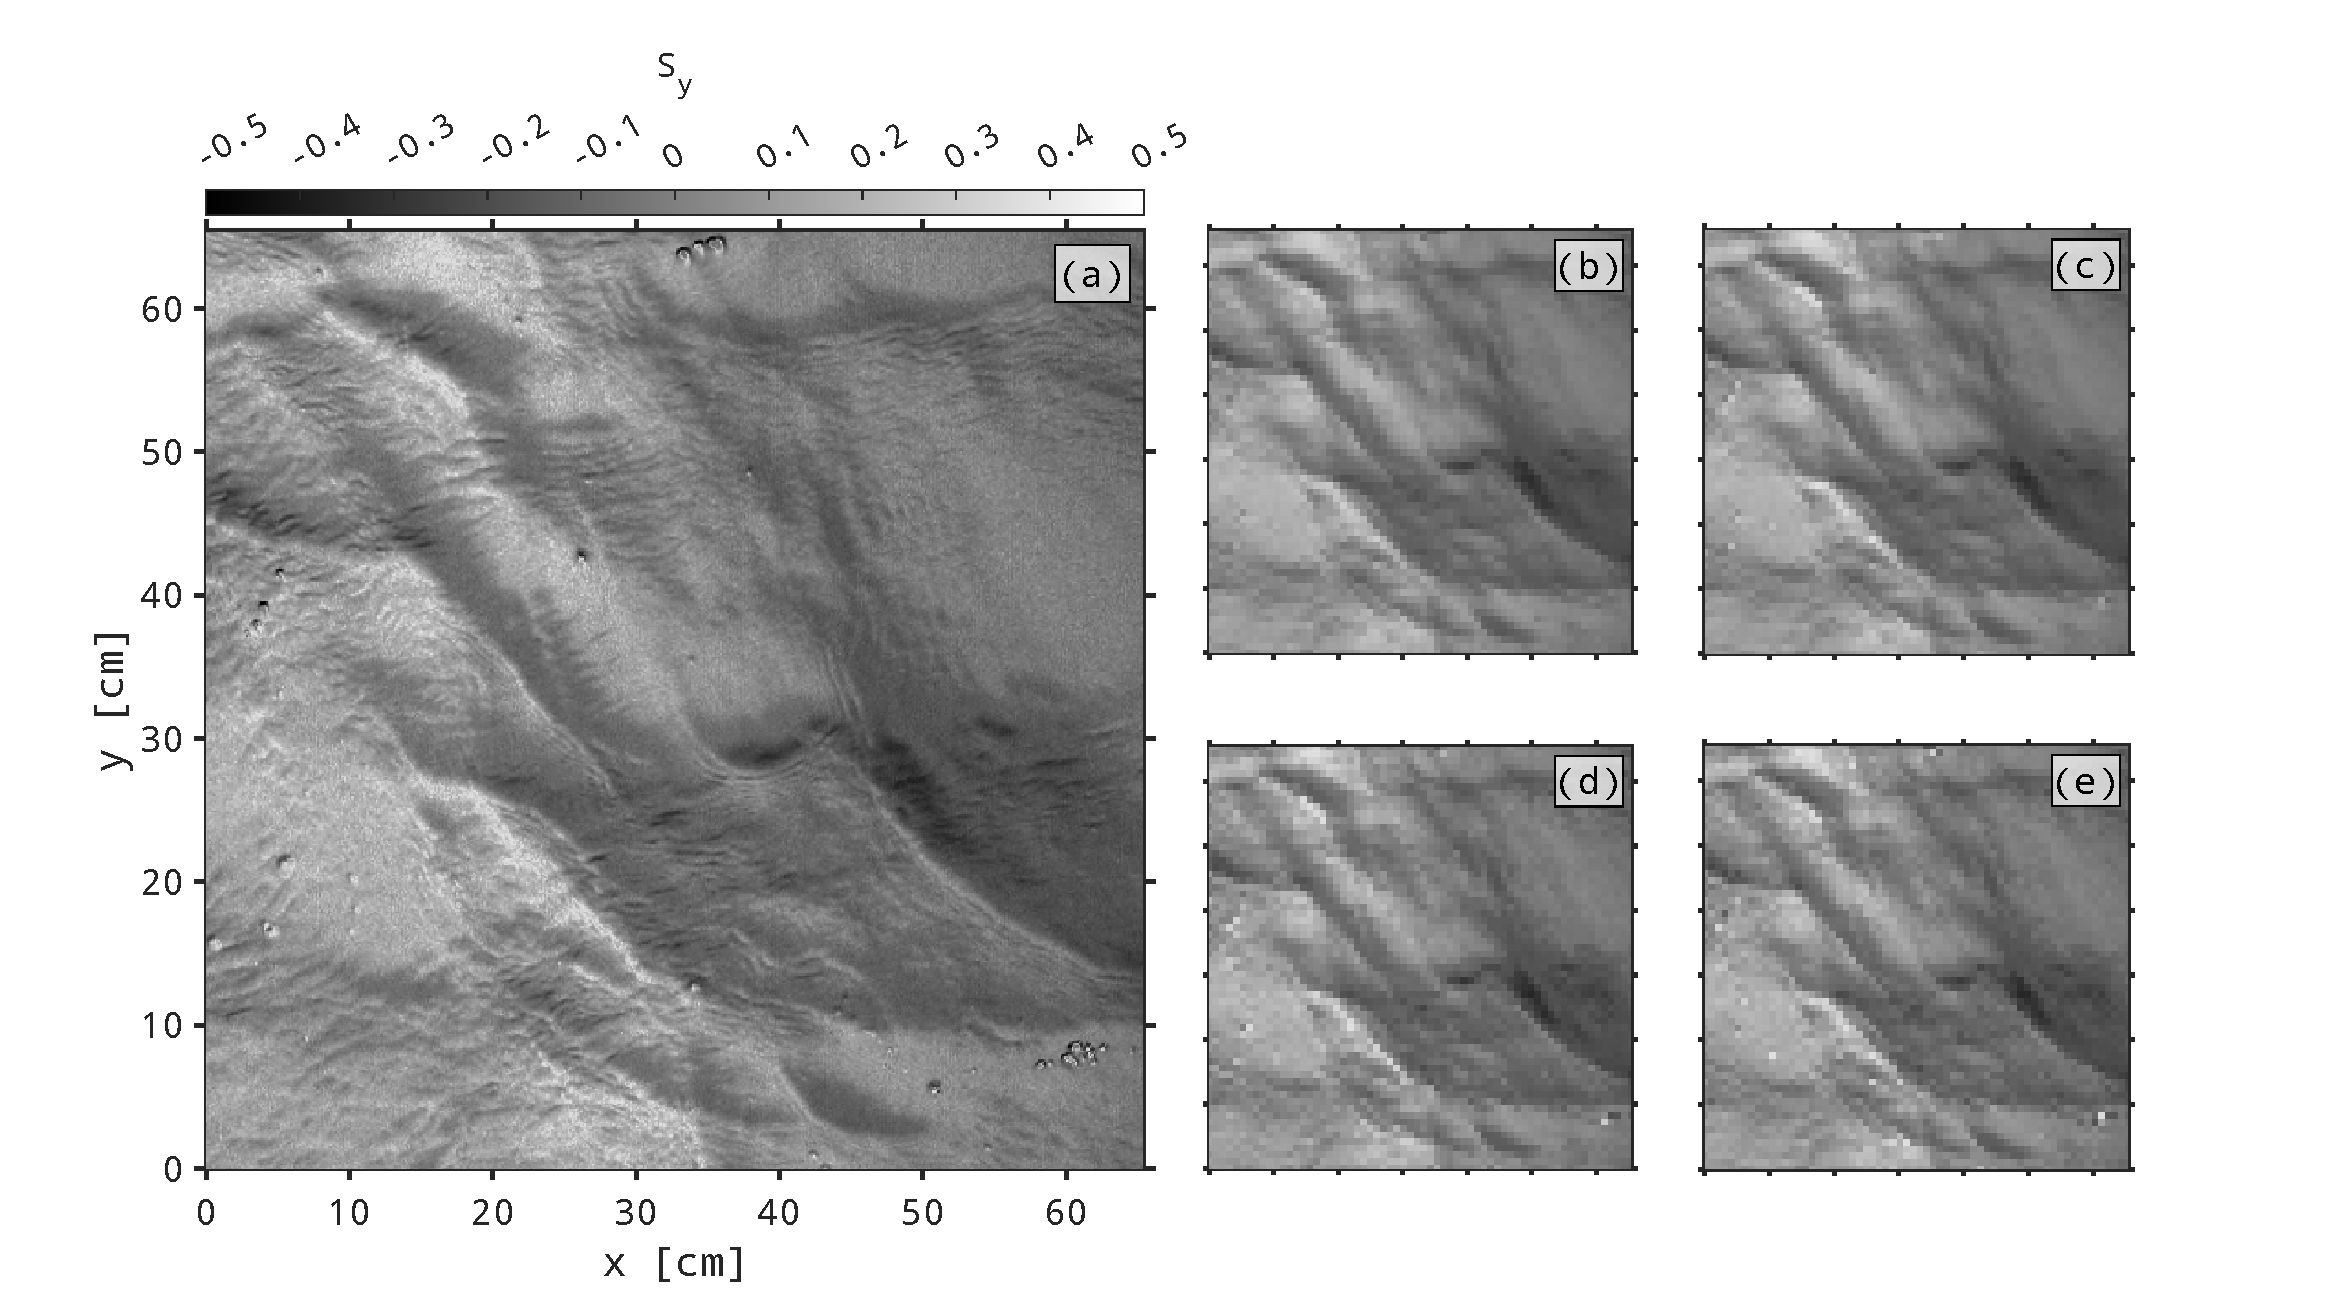
\includegraphics[width=\textwidth]{_figures/slopefield_full_degraded_examples.pdf}
% \vspace{-20pt}
% \caption{Along-look (y) component of a water slope field obtained from a DoAm polarimeter during RaDyO 2008 \cite{Zappa2012,Laxague2018b}: (a) full resolution and degraded through averaging at the level of either (b) slope or (c) intensity. An additional step involved imitation of a DoFP detector design and use of either (d) bilinear interpolation or (e) a 12-pixel kernel \cite{ratliff_interpolation_2009}. Despite size differences, all frames extend over the same spatial footprint: $\approx$ 67 cm $\times$ 67 cm.}
% \label{fig:slopefield_full_degraded_examples}
% \end{figure*}

% Generally speaking, investigations into the performance or fidelity of an observational technique require an external standard as a reference point. Our investigation in particular requires that this external standard be of higher spatial resolution than the observations under scrutiny-- a tall order given the exceptional (order 1 mm) resolution of existing PSS field datasets \cite{Zappa2012,Laxague2015,Laxague2018b}. We determined that the best approach would involve a combination of field observational datasets---collected from different sensor types---and numerical modeling, allowing us to address each of our driving questions in isolation. This approach was divided into three distinct activities:
% \begin{enumerate}[label=(\Alph*)]
%     \item Generation of a synthetic sea surface at sub-millimeter resolution, followed by implementation of a polarization-aware ray-tracing model to produce simulated fields of the Stokes parameters, yielding surface angles $\theta$ and $\varphi$.
%     \item Block-averaging of data collected via DoFP detector---either at the level of raw polarized light intensity or at the level of the computed slope field---for the purpose of simulating an increase in pixel spatial size.
%     \item Use of a high-resolution DoAm detector to obtain spatially collocated polarization information, modifying processing to mimic the sparse information of the DoFP detector.
% \end{enumerate}

% Activities A \& B provided a means for investigation of our first concern (\lq\lq Spatial averaging of polarization state is not necessarily equivalent to spatial averaging of surface orientation"). Activity C enabled the interrogation of our second concern (\lq\lq Polarization intensity measurements made by DoFP polarimeters are spatially sparse (non-collocated).") by way of the DoAm polarimeter's spatially dense measurement.

% \newpage

% \subsection{Modeling Light Reflection From a Synthetic Sea Surface}

% Our procedure for generation of a synthetic sea surface and modeling light reflection from that surface follows a long-standing combination of methods which have been used to great success in electronic entertainment industries \cite{tessendorf_simulating_2001} and is emerging as a powerful tool for investigation of problems relevant to remote sensing of surface waves \cite{dalimonte_effects_2016,xue_airborne_2021}:

% \begin{enumerate}
%     \item We applied a random phase approach to the simulation of a realistic sea surface \cite{tessendorf_simulating_2001}; see the left panel of Figure \ref{fig:synthetic_surface_DoLP_ORI}. In this case, the wavenumber directional spectrum of Elfouhaily \emph{et al.} [1997] \cite{Elfouhaily1997} was chosen because it yields the long wave characteristics of JONSWAP-type spectra while constraining the high-wavenumber behavior to reproduce the short wave slope statistics first observed by Cox \& Munk \cite{Cox1958}.
%     \item We executed a simple ray-tracing model to compute the change in polarization state of light reflected from our simulated sea surface \cite{mobley_polarized_2015}. Our implementation of this model reverses the order of light propagation, treating an artificial pinhole camera as the source of rays oriented at the simulated sea surface. Given knowledge of the relative orientation of the incident ray and the surface normal, the Stokes parameters at that point in the field of view are computed via Mueller calculus (Figure \ref{fig:light_reflection_demonstration}).
% \end{enumerate}

% These simulations were run at 12 wind speeds: [3:1:14] m s$^{-1}$ on 8192 $\times$ 8192 arrays with $3.14\times$10$^{-4}$ m px$^{-1}$ spatial resolution (Nyquist wavenumber $k_{Nyq}=$ 10$^4$ rad m$^{-1}$). The simulation was repeated ten times per wind speed with new phase information to provide a larger sample size for the comparisons.

% We offer a few caveats relevant to this approach. First: although waves in our simulation obey the gravity-capillary dispersion relation, there are no additional hydrodynamic constraints to enforce wave current interactions and the resulting parasitic capillary waves \cite{Fedorov1998a} or phase-locked bound waves \cite{Plant1999a}. For this reason, we refrain from making 1:1 comparisons between the statistical results produced from our simulations and those obtained from field observations of real sea surfaces. 

% \begin{figure*}[!hb]
% \centering
% 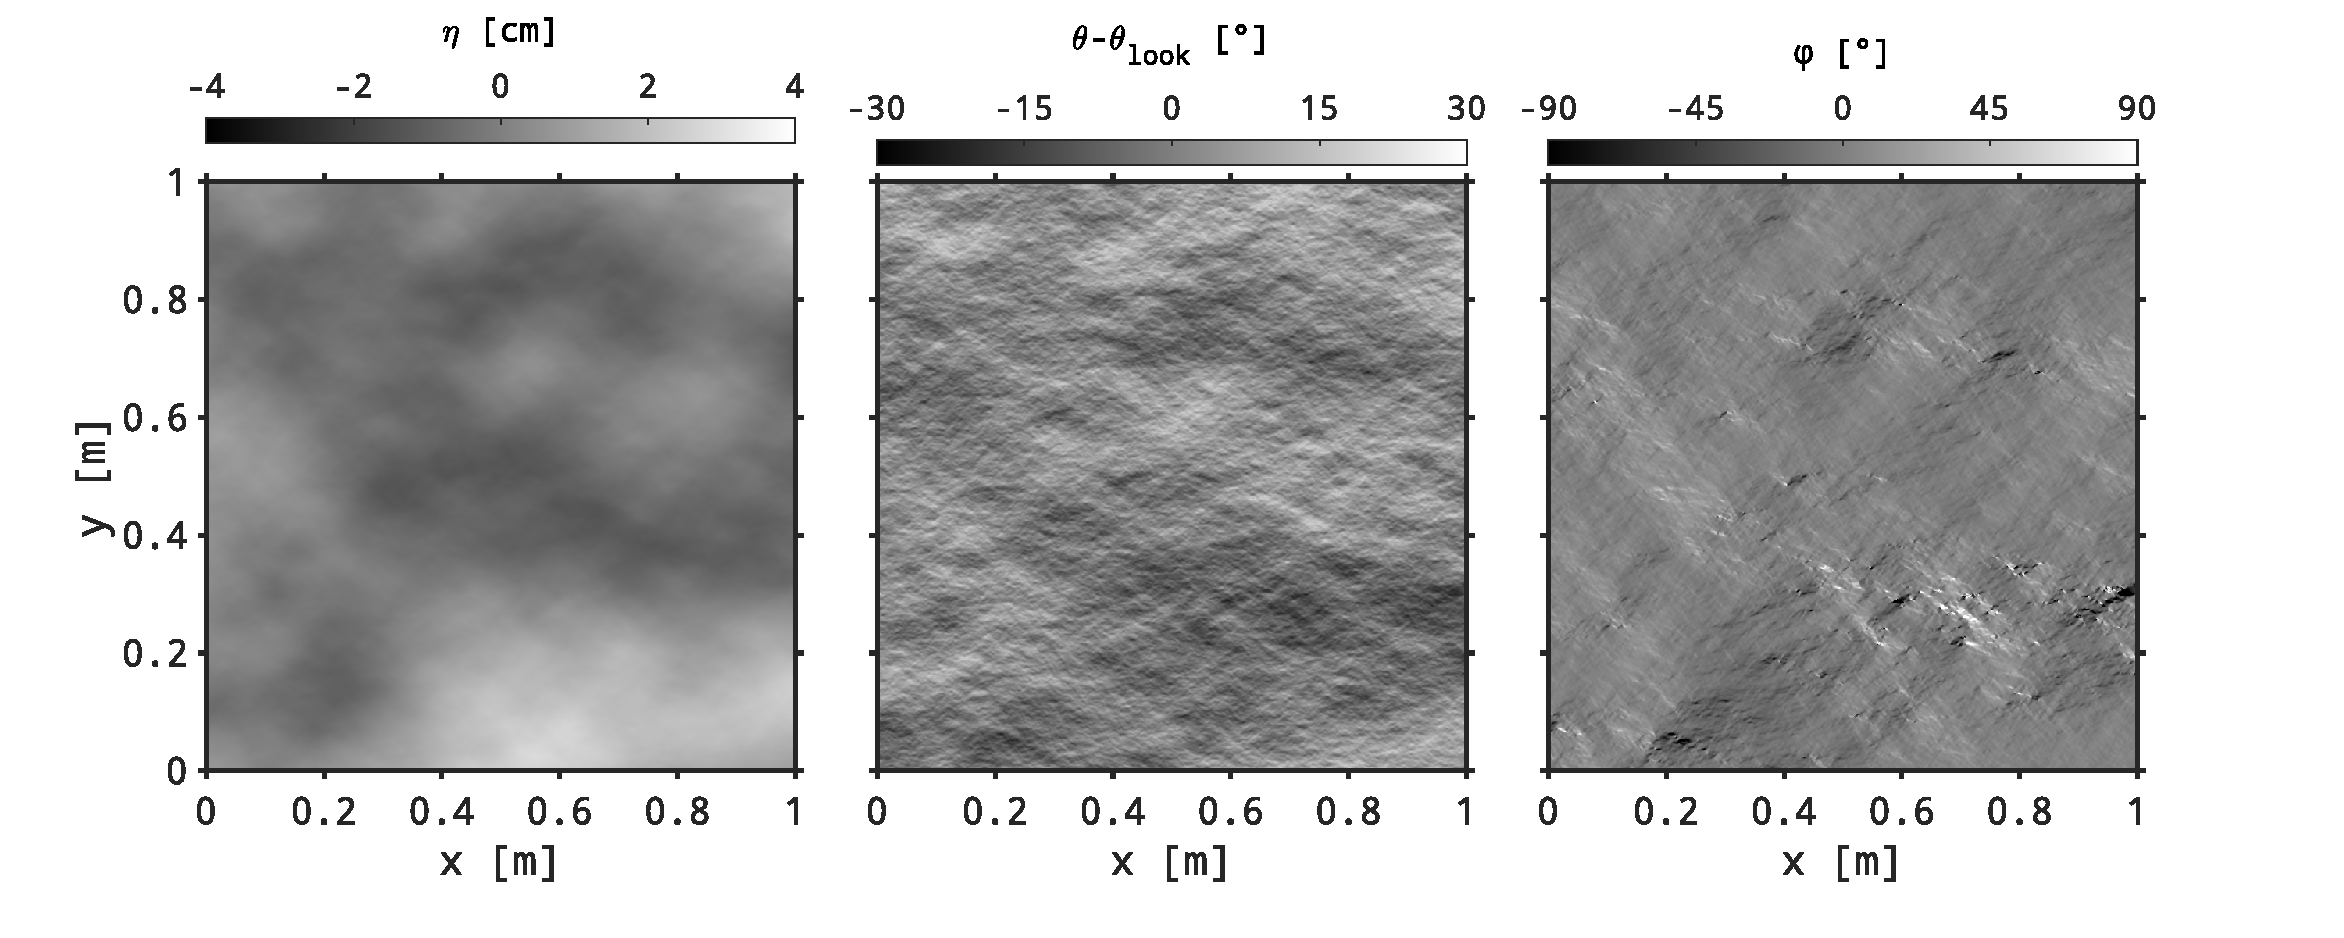
\includegraphics[width=\textwidth]{_figures/synthetic_surface_DoLP_ORI.pdf}
% \vspace{-30pt}
% \caption{Left panel: synthetic surface produced via wavenumber directional spectrum \cite{Elfouhaily1997} and random phase approach \cite{tessendorf_simulating_2001}. The middle and right panels respectively show $\theta$ and $\varphi$ of modeled light reflected from this simulated surface \cite{mobley_polarized_2015}.}
% \label{fig:synthetic_surface_DoLP_ORI}
% \end{figure*}

% \newpage

% \begin{figure}[!ht]
% \centering
% 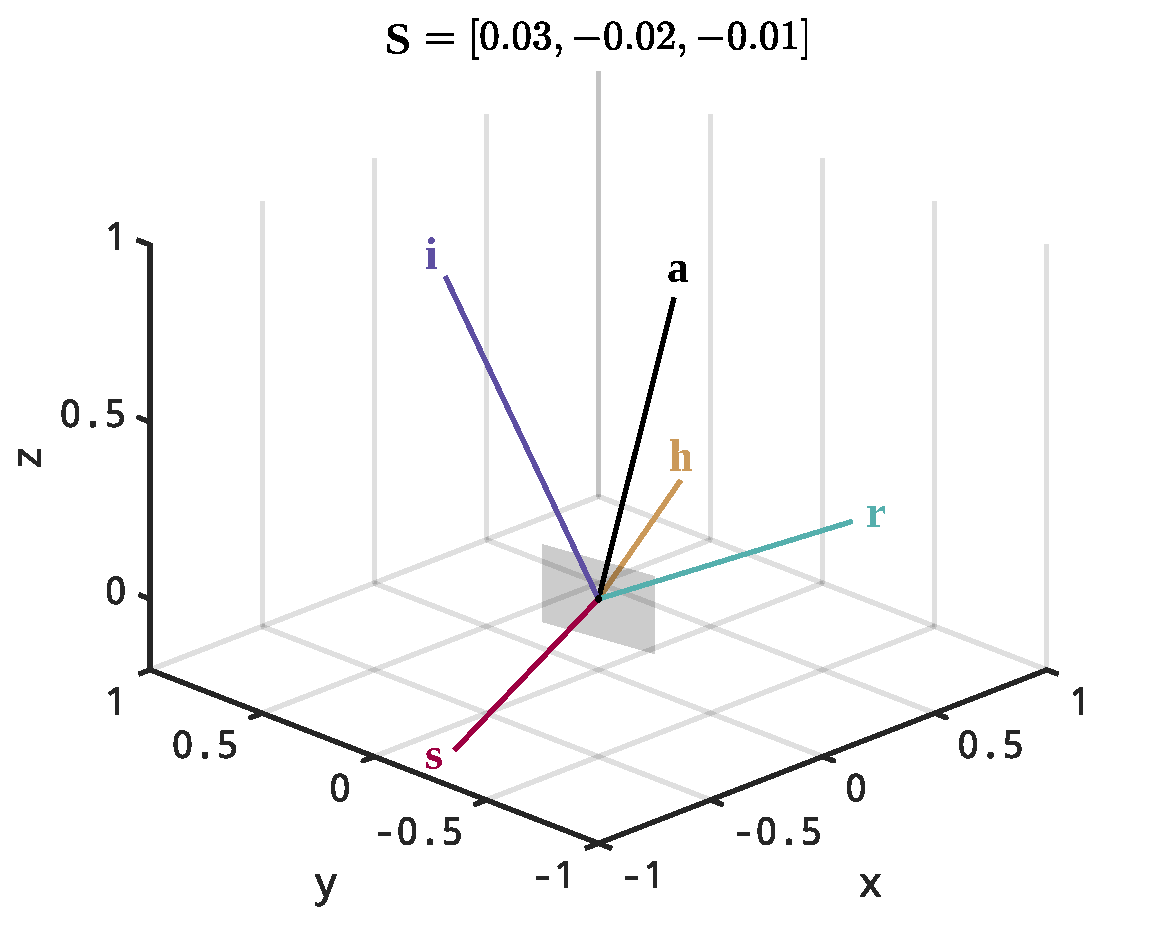
\includegraphics[width=0.48\textwidth]{_figures/light_reflection_demonstration.pdf}
% \caption{Simulation of light reflected from a facet oriented with a slope vector of [0.01,0.37]. The vectors $\textbf{a}$, $\textbf{i}$, and $\textbf{r}$ represent the surface normal, the incident ray, and the reflected ray, respectively. The vectors $\textbf{h}$ and $\textbf{s}$ represent two byproducts which are used in the calculation of the polarization state of the reflected light \cite{mobley_polarized_2015}: a Stokes vector of $\textbf{S}=$[0.03,-0.02,-0.01].}
% \label{fig:light_reflection_demonstration}
% \end{figure}

% \vspace{-7pt}

% Second: we have assumed that sky-leaving radiance is unpolarized, the result of which simplifies the calculations and eliminates the need for sky-leaving polarization measurements. Such an assumption is often made in real-world observations \cite{Zappa2008,Laxague2015}, though its validity strongly depends on ambient illumination/weather conditions \cite{goldstein_polarized_2017,voss_polarized_1997}. We expect that a uniform slope bias would be the principal result of polarized sky-leaving radiance. Finally, we have neglected all effects associated with surface-leaving (upwelling) radiance. This assumption is often made for field observations, though it is not universally safe to do so \cite{You2011,ibrahim_relationship_2012}. Surface-leaving radiance is expected to be mostly depolarized due to scattering within the water column, resulting in a lower signal-to-noise ratio. However, the pixel-scale effects at the focus of the present manuscript are expected to exist regardless of these known challenges associated with PSS, and as such we do not discuss them further here.

% \newpage

% \subsection{Block Averaging: Intensity or Slope}

% To address the first concern, regarding the spatial averaging of polarization state and surface orientation, we choose angle of incidence $\theta$ and polarization orientation $\varphi$ as variables for comparison. Going beyond Stokes parameters or DoLP allows for easier interpretation of results (e.g., one can easily conceptualize a 1$^{\circ}$ error; the same can't be said for error in DoLP of 0.02). Stopping short of the slope field components $\mathcal{S}_x$ and $\mathcal{S}_y$ allows us to make our comparison in the frame of reference of the reflecting plane, before $\theta$ and $\varphi$ are entangled (i.e., as in equation \ref{eq:from_angle_to_slope}). We leverage field measurements of polarization intensity and the light reflection model on the simulated surface to compare the results of spatial averages of polarization state and surface orientation. Spatial averaging is done by block-averaging, where the mean value of n$\times$n blocks of pixels is computed to produce an image of degraded spatial resolution. 
% With field measurements of polarization state, we compare low spatial resolution $\theta$ and $\varphi$ fields as computed two ways, as summarized in the right-hand-side of Figure \ref{fig:slope_intensity_degradation_flowchart}. In the first method, $\theta$ and $\varphi$ are computed from the measured intensity and then the resolution is degraded (Figure \ref{fig:slope_intensity_degradation_flowchart} lower right-to-left), and in the second method, the measured intensity is degraded and then $\theta$ and $\varphi$ are computed (Figure \ref{fig:slope_intensity_degradation_flowchart} upper right-to-left). 
% With simulated slope fields and the light reflection model, two methods of computing low resolution $\theta$ and $\varphi$ are also summarized in 
%  Figure \ref{fig:slope_intensity_degradation_flowchart}. In one, high resolution $\theta$ and $\varphi$ are simulated from the slopes with the reflection model and then the resolution is degraded (Figure \ref{fig:slope_intensity_degradation_flowchart} lower left-to-right). In the other, the simulated slope is degraded to a lower resolution and then $\theta$ and $\varphi$ are simulated with the reflection model (Figure \ref{fig:slope_intensity_degradation_flowchart} upper left-to-right). 

% \begin{figure*}[!hb]
% \centering
% 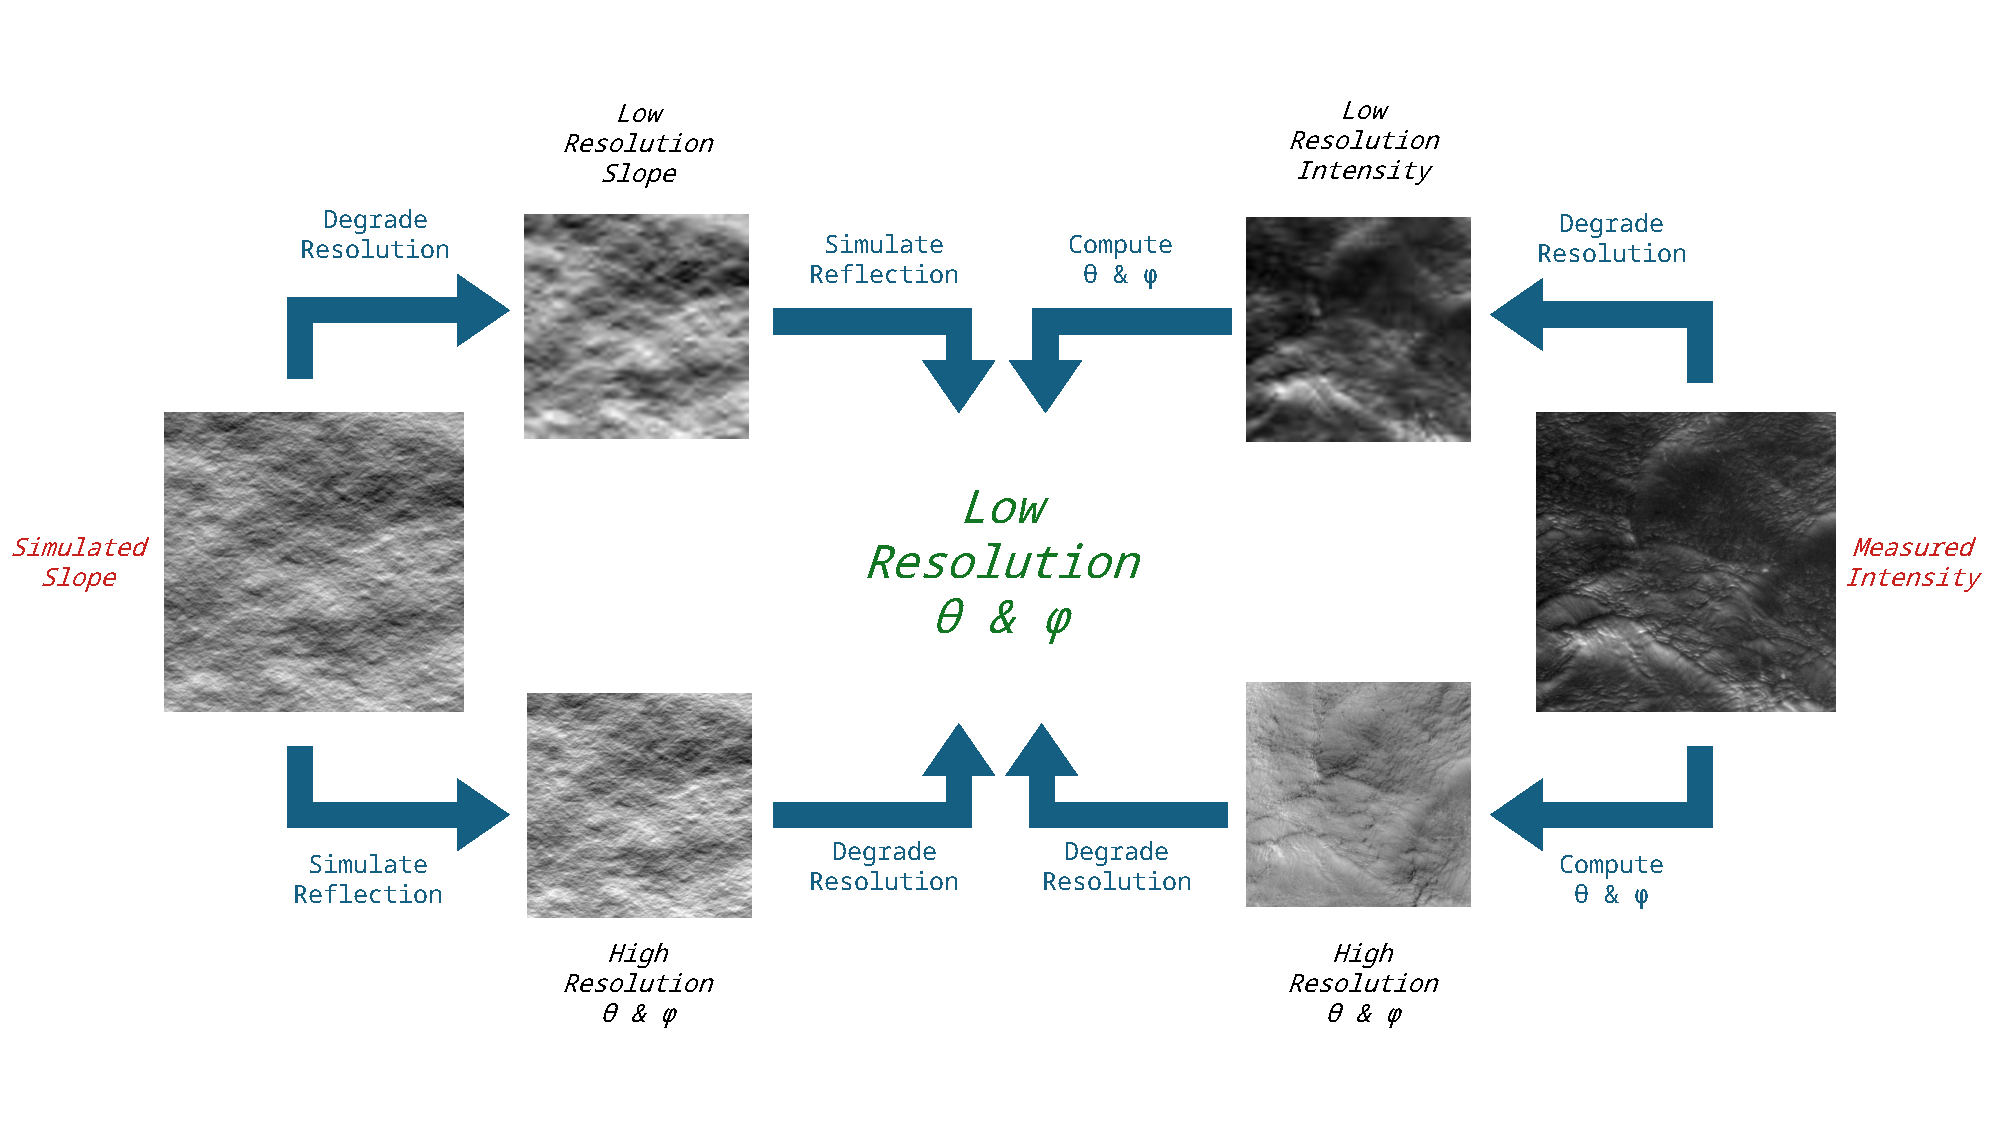
\includegraphics[width=1\textwidth]{_figures/slope_intensity_degradation_flowchart.pdf}
% \vspace{-20pt}
% \caption{Flowchart representing strategies for investigating the effects of reduced resolution on the measurement of surface slope. For our simulated surface/reflection approach, we start from the left of the flowchart; for our field observational approach, we start from the right of the flowchart.}
% \label{fig:slope_intensity_degradation_flowchart}
% \end{figure*}

% \newpage

% \subsection{Applying DoFP Processing to DoAm Data}

% Investigation of our second concern (regarding the sparseness of the individual intensity measurements made via DoFP) requires a source dataset which was obtained with a non-DoFP detector at exceptionally high spatial resolution ($\approx$1 mm px$^{-1}$). We chose the dataset obtained during the 2008 RaDyO field campaign \cite{Zappa2012,Laxague2018b}. The polarimeter used during that campaign was a custom-built DoAm device with a specialized optical path and four CCD cameras. After laboratory calibration via integrating sphere and external polarizing filter \cite{powell_calibration_2013}, a data reduction matrix was produced which allowed for calculation of $I_{0}$, $I_{45}$, $I_{90}$, and $I_{135}$ at each pixel within a 768 $\times$ 576 array at a sample rate of 60 frames per second. For that deployment aboard \emph{R/P FLIP}, the 4.8$^{\circ}$ $\times$ 3.6$^{\circ}$ field of view yielded footprint of 1-1.25 m in diameter with approximately 1.5 mm per pixel. A detailed description of the short wave measurements made during RaDyO 2008 is available elsewhere \cite{Zappa2012,Laxague2018b}.

% Our reprocessing of this dataset involved an intentional and specific degradation to mimic the spatially sparse observations made by a DoFP detector. In this process, arrays of the full-frame intensity fields obtained via DoAm were subjected to spatially-offset subsampling (as in the middle panel of Figure \ref{fig:DoFP_superpixel_and_interpolation}) before bilinear interpolation to recover four new intensity arrays (as in the right panel of Figure \ref{fig:DoFP_superpixel_and_interpolation}). Tradeoffs exist with this approach. On the one hand, interpolation is intended to mitigate negative effects associated with the sparse, non-collocated observations. On the other, each of these new arrays contain 25\% of the information of their source arrays, so care must be taken to avoid attributing too much meaning to the high-wavenumber behavior of the computed slope fields.

% \newpage

% \subsection{Spatial averaging of polarization state}
% \label{sec:results_spatial_averaging}

% \begin{figure*}[!hb]
% \centering
% 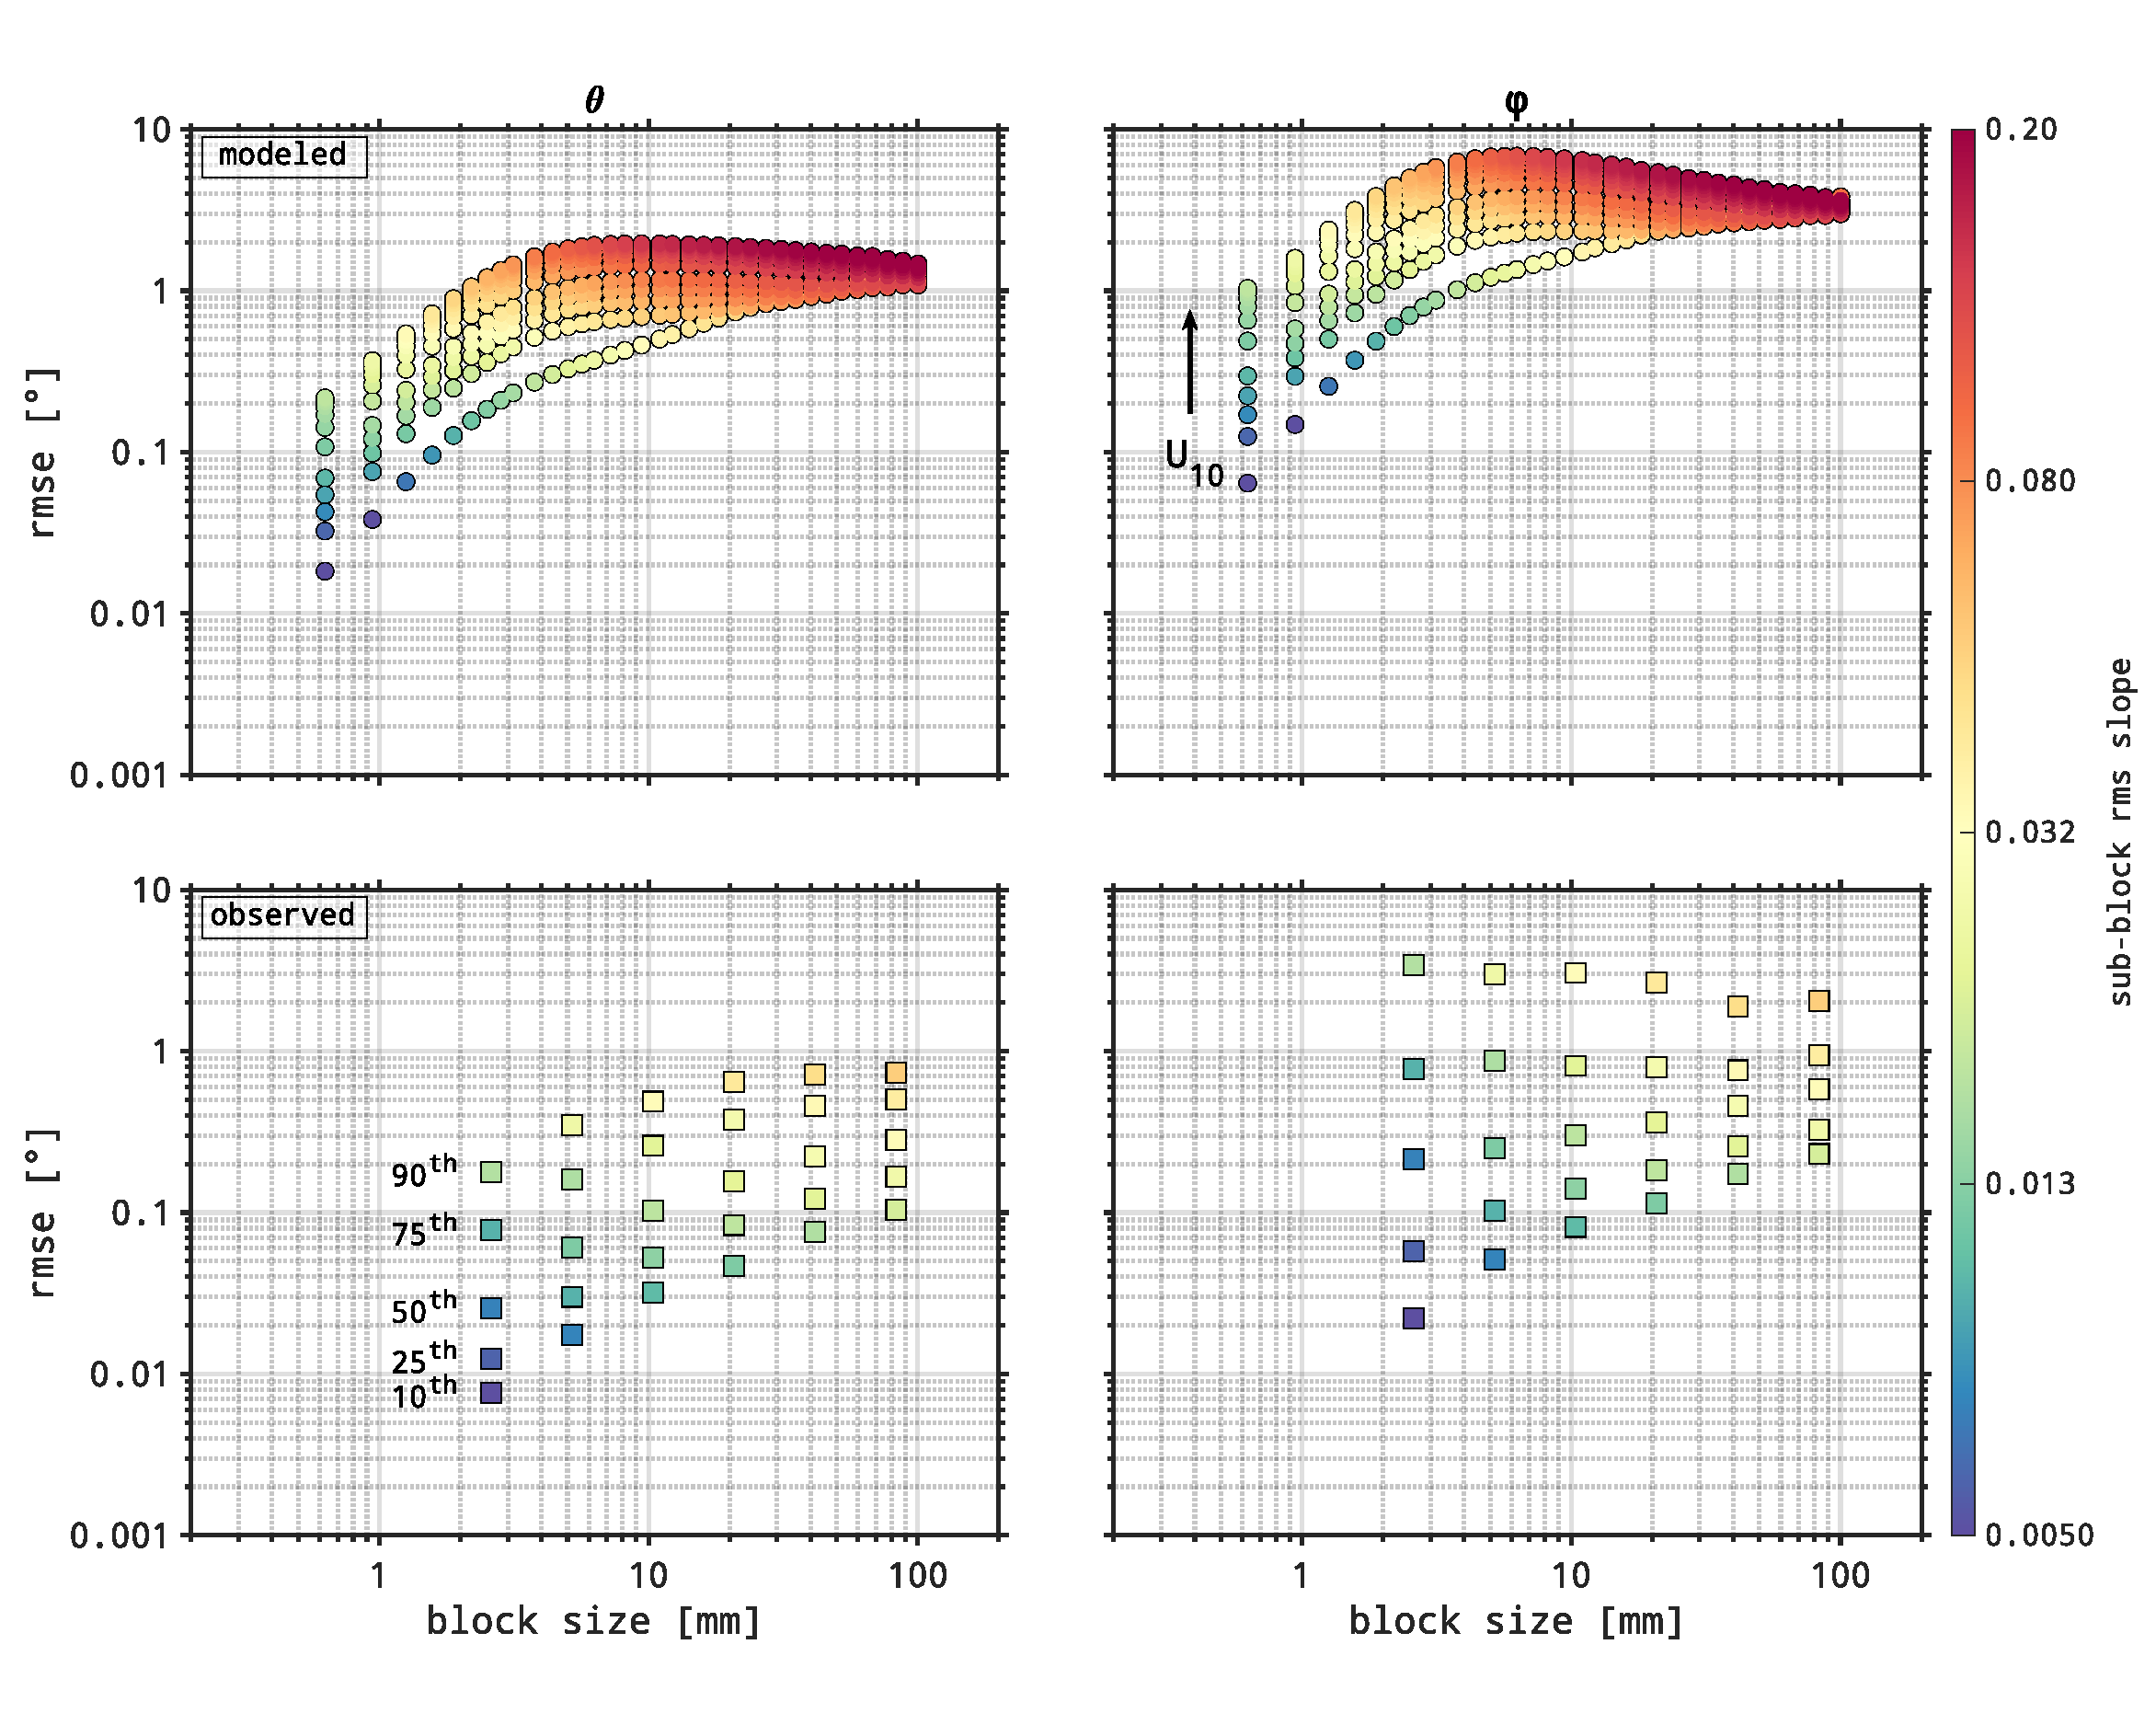
\includegraphics[width=1\textwidth]{_figures/simulated_and_ASIT_surface_angle_RMSE.pdf}
% \caption{Root-mean-square error (RMSE) for incidence angle ($\theta$) and polarization orientation angle ($\varphi$) computed from light reflected off simulated surface. Color indicates sub-block root-mean-square slope. Top row contains results from simulation, with increasing vertical levels corresponding to input wind speed; bottom row contains results from ASIT field campaign, with increasing vertical levels corresponding to percentile ranges in RMSE.}
% \label{fig:simulated_and_ASIT_surface_angle_RMSE}
% \end{figure*}

% The first quantitative comparison we make follows our permutation of the order of spatial averaging (polarization vs. slope, e.g.) as represented in the flowchart of Figure \ref{fig:slope_intensity_degradation_flowchart}. Specifically, we compare the surface angles $\theta$ and $\varphi$ computed from full-resolution fields (and then averaged in space) to the surface angles computed from slope fields which have themselves been averaged in space. We chose the root-mean-square error (RMSE) as our metric for performing this comparison. RMSE retains the units of the input variable (e.g., in contrast with the coefficient of determination $R^2$ or the $p$-value of a 1:1 linear comparison). Furthermore, RMSE provides information about point-to-point variation even if the difference is zero on average, making the metric superior to mean absolute error for our purposes here. The comparison was executed by computing the point-by-point difference in free surface angle ($\theta$ or $\varphi$) for a given wind speed, squaring that difference, computing the average over all space (and across all ensemble members), and then performing the square root of the resulting quantity.

% This comparison was performed on the outputs of simulations of the sea surface at 12 wind speeds (from 3 m s$^{-1}$ to 14 m s$^{-1}$ in increments of 1 m s$^{-1}$); an ensemble of ten unique realizations of the sea surface was generated for each wind speed. An analogous comparison was performed on a set of DoFP field observations made in 2019 at the Air-Sea Interaction Tower (ASIT) south of Martha's Vineyard, MA ($N =$ 70, 1 m s$^{-1}\leq U_{10}\leq$12 m s$^{-1}$).

% Results of this process are shown in Figure \ref{fig:simulated_and_ASIT_surface_angle_RMSE}: the top and bottom rows contain results from the simulation and field observations, respectively. The markers on these panels have been colored by the root-mean-square (RMS) slope of surface waves smaller than the scale of the block average (e.g., at the sub-block). A graphic to aid in the interpretation of this quantity is given in Appendix \ref{sec:appendix_subpixel_rms_slope}, where Figure \ref{fig:subpixel_RMS_slope} provides sub-block RMS slope as a function of block size (or cutoff wavelength) for spectra \cite{Elfouhaily1997} produced over a range of wind speeds.

% \newpage

% \begin{figure}[!ht]
% \centering
% 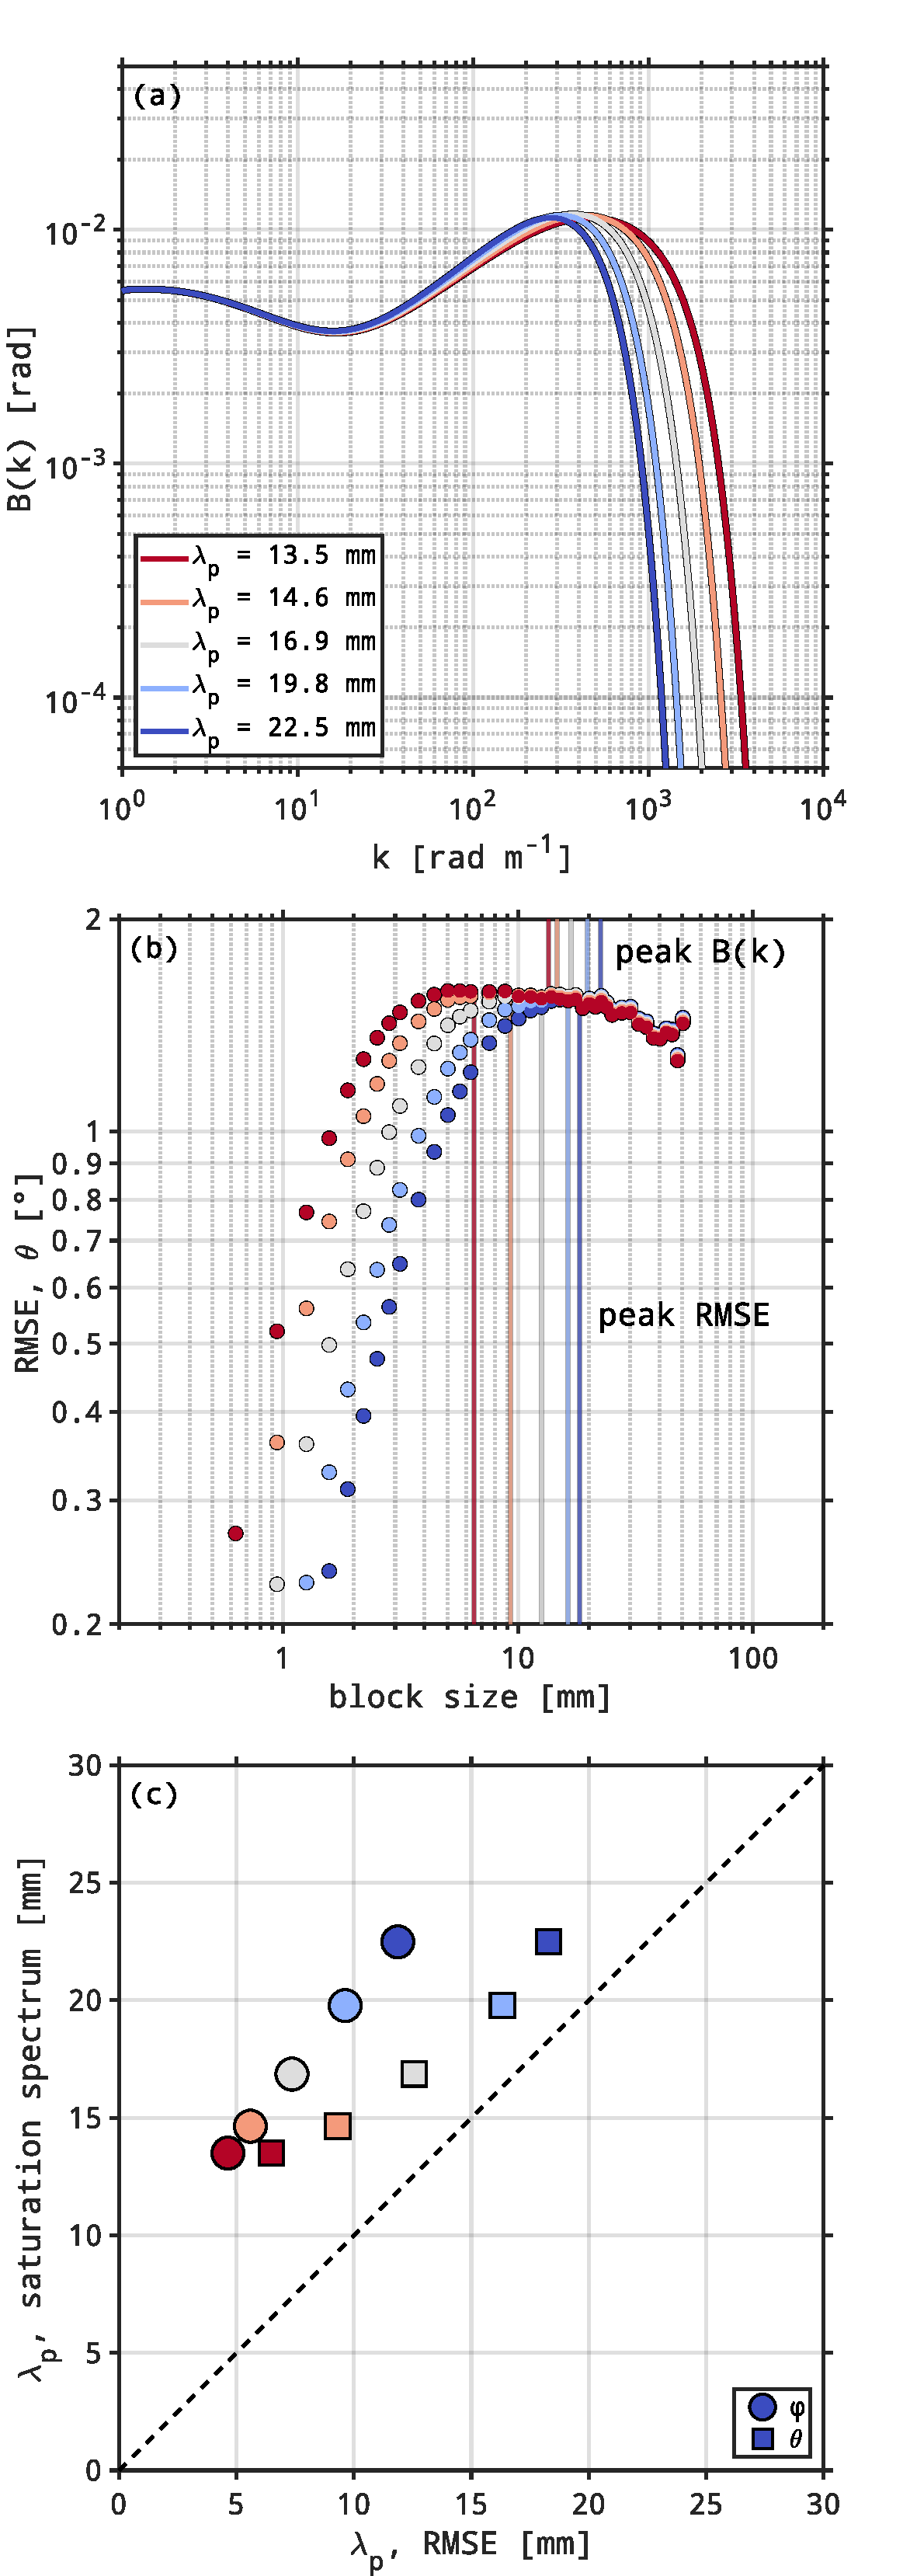
\includegraphics[width=0.43\textwidth]{_figures/spectral_nudge_3panel.pdf}
% \vspace{-5pt}
% \caption{(a) Wavenumber saturation spectra \cite{Elfouhaily1997} generated for $U_{10}=$ 10 m s$^{-1}$, with short wave peak shifted up/down by $\pm$15\% and $\pm$25\%. (b) Corresponding RMSE in computed interfacial incidence angle $\theta$; vertical lines connect short wave spectral peak to scale peak of RMSE output. (c) 1:1 scatterplot of peak lengthscales from RMSE and saturation spectrum.}
% \label{fig:spectral_nudge_3panel}
% \end{figure}

% \newpage

% In our simulations, RMSE angle increased monotonically with wind speed, saturating at higher levels of forcing (U$_{10}\gtrapprox$ 8 m s$^{-1}$). Furthermore, error increased substantially with block size before peaking at 5-10 mm and then weakly rolling off for larger averaging regions. This behavior will be discussed at greater length in section \ref{sec:discussion}. For the sake of clarity, RMSE angle obtained from the field observations has been reported at five quantiles (10$^{\mathrm{th}}$, 25$^{\mathrm{th}}$, 50$^{\mathrm{th}}$, 75$^{\mathrm{th}}$, \& 90$^{\mathrm{th}}$ percentiles) for each of the six block sizes. This distillation provides a simple view of the mean behavior and variation of RMSE angle and preserves the salience of sub-block RMS slope. In these observations, we found RMSE in $\theta$ to exhibit strong variation with block size in contrast to the weak variation with block size of $\varphi$ varied weakly with block size. For both angles, RMSE was found to increase with sub-block RMS slope for a particular block size.

% It is apparent that for any given block size, the sub-block RMS slope obtained from ASIT field observations is substantially lower than the corresponding value in the simulation. This is not a bias in the forcing regime: both the simulation and the field observations span an analogous range in wind speed. One reasonable explanation for the disparity lies in the differing resolutions between the simulation ($\approx$0.3 mm px$^{-1}$) and field observations ($\approx$1.1 mm px$^{-1}$). Another reasonable explanation is associated with the model spectrum used in our simulations \cite{Elfouhaily1997}. This spectrum is generally considered to be \emph{the} standard reference in the field of remote sensing of the ocean surface. However, no model spectrum provides a perfect realization of the ocean surface at every scale, a shortcoming that is particularly salient at high wavenumbers, where there remains significant variability between and among models and field observations \cite{Hara1998a,Yurovskaya2013,Hwang2015,Laxague2015,Laxague2018b}.

% One of the distinguishing qualitative features of the Elfouhaily \emph{et al.} \cite{Elfouhaily1997} saturation spectrum is its one short wave peak at $k=$ 370 rad m$^{-1}$ ($\lambda=$17 cm, $c=$ 23 cm s$^{-1}$) which does not vary with wind speed or fetch. The simulation results presented in Figure \ref{fig:simulated_and_ASIT_surface_angle_RMSE}a,b indicate the existence of a single peak value of RMSE at a block size of approximately 5-10 mm. In order to investigate the degree to which variation of RMSE with block size in our simulations is contingent upon the short wave sea state, we performed artificial \lq\lq nudges" of the model spectral peak. These nudges are presented in Figure \ref{fig:spectral_nudge_3panel}a, which contains the original spectrum (light gray curve) and the nudged (red/blue curves) spectra (peak wavenumbers are provided in the form of wavelengths within the figure caption). The synthetic water surfaces produced from these spectra were subjected to the same sequence of processing outlined in Figure \ref{fig:slope_intensity_degradation_flowchart}, yielding the RMSE in $\theta$ as a function of block size (Figure \ref{fig:spectral_nudge_3panel}b). Indeed: the scale at which peak angular error occurs is positively correlated with the scale of the saturation spectral peak, with the spectral peak being uniformly larger than the RMSE peak (Figure \ref{fig:spectral_nudge_3panel}c).

% \newpage

% \begin{figure}[!ht]
% \centering
% 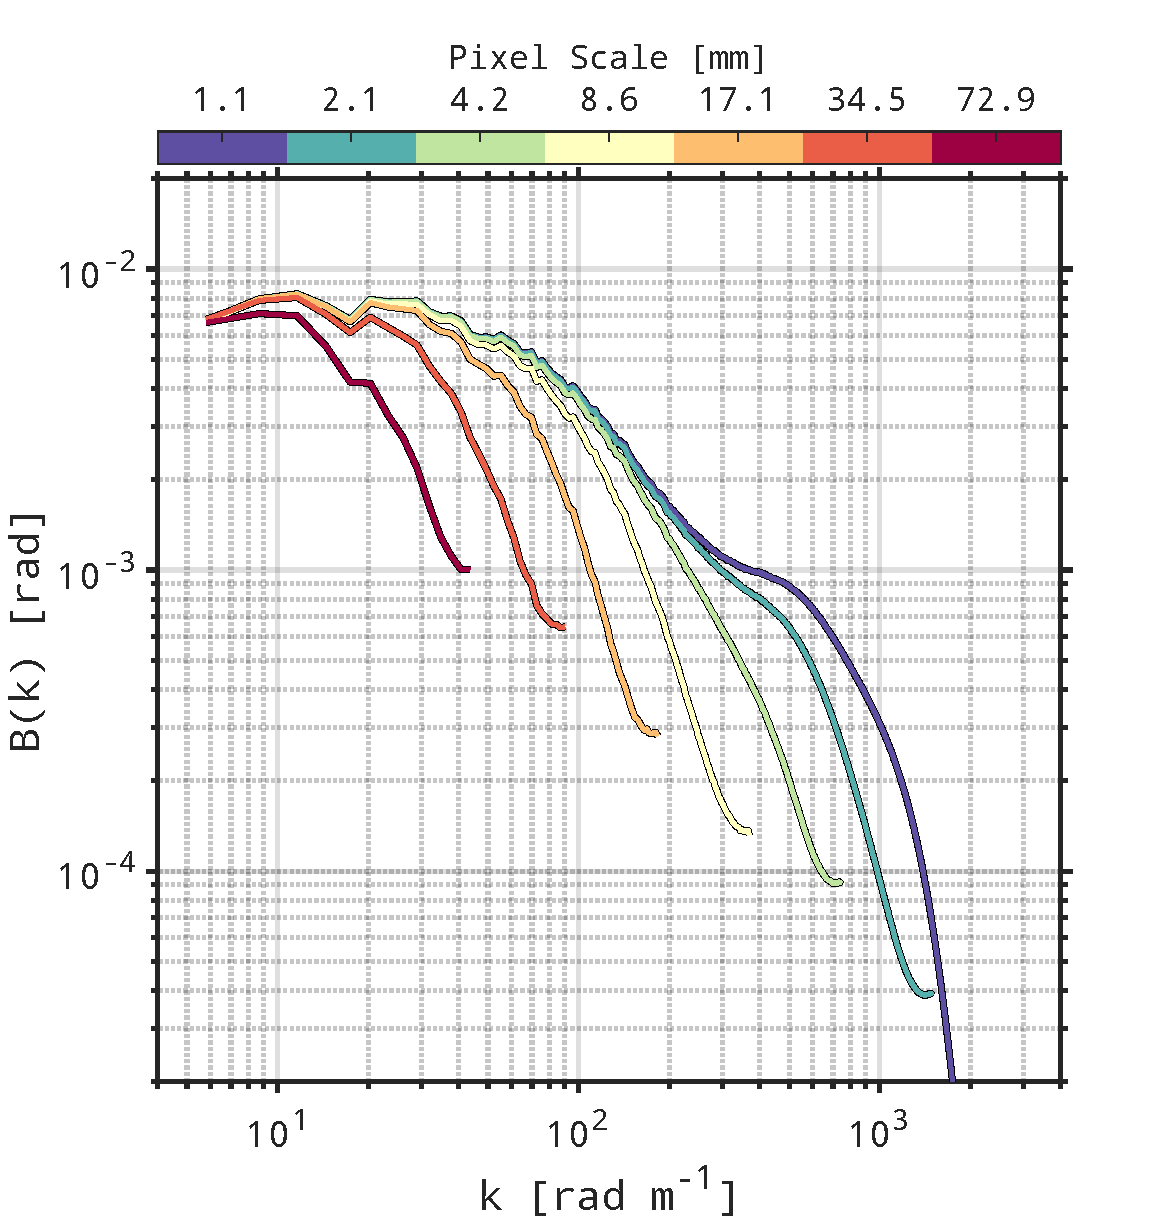
\includegraphics[width=0.5\textwidth]{_figures/block_averaged_ASIT_spectra.pdf}
% \vspace{-20pt}
% \caption{Omnidirectional wavenumber saturation spectra for a particular case ($u_*=$ 15.9 cm s$^{-1}$). Color indicates the size of the block average applied to the intensities before calculation of the slope fields. The violet curve (1.1 mm pixel size) represents the spectrum computed from the full-resolution slope fields.}
% \label{fig:block_averaged_ASIT_spectra}
% \end{figure}

% Our next step of analysis involved examining the effect of spatial averaging of polarization intensities on the wave slope/saturation spectra. This was accomplished by comparing spectra computed from slope fields produced from the measured polarization intensities (with a pixel scale of 1.1 mm) to spectra computed from slope fields produced from spatially-averaged polarization intensities (with pixel scales of 1.1 $\times$ $N$ mm, where $N$ $\times$ $N$ pixels were block-averaged). It is important to note that these measurements were taken with a DoFP sensor, so the scale simulated by 2 $\times$ 2 block averaging is the same scale of the superpixels of the original measurement. A representative example is shown in Figure \ref{fig:block_averaged_ASIT_spectra}. The Nyquist wavenumber is, by definition, halved by doubling the pixel scale. However, an additional consequence of spatial averaging is that the spectral intensity is diminished relative to the full-resolution spectrum at scales much larger (wavenumbers much less) than the Nyquist wavenumber. Spectral intensity, and thus contribution to the total mean square slope, is lost not only beyond the Nyquist wavenumber, but also within the resolved scales. In cases when there is a significant spectral peak at high wavenumbers corresponding to wind-driven capillary waves, spatial averaging diminishes the peak despite resolving waves at that scale. 

% We quantify this loss of spectral density with the percent difference between the spectra computed from slopes produced via full-resolution intensity fields and the spectra computed from the slopes produced via spatially-averaged intensity fields.

% \newpage

% We then compute a normalized reference wavenumber $k^*$ defined such that $k^*$ varies from 0 to 1 for all block sizes.
% \begin{equation}
% \label{eq:k_star_definition}
%     k^*\equiv\frac{k-k_{min}}{k_{max}-k_{min}}
% \end{equation}
% The percent difference between the original spectra and the spatially-averaged spectra collapses along all pixel scales with this normalization, as shown in Figure \ref{fig:block_averaged_ASIT_spectra_normalized}a. The spectral energy is diminished by 20\% at $k^* = 0.2$ (at approximately 20\% of the Nyquist wavenumber), and 80\% of the original spectral intensity is lost at $k^* = 0.7$. We extend this analysis to the range of wind conditions captured in the ASIT dataset in  Figure \ref{fig:block_averaged_ASIT_spectra_normalized}b. The percent difference between the the original spectra and the spatially-averaged spectra at one scale for all cases is conditionally averaged by friction velocity. Little variation is observed among wind conditions, suggesting that the behavior of spectra from spatially averaged intensities is not impacted by pixel scale or by wind forcing. 

% \begin{figure}[!hb]
% \centering
% 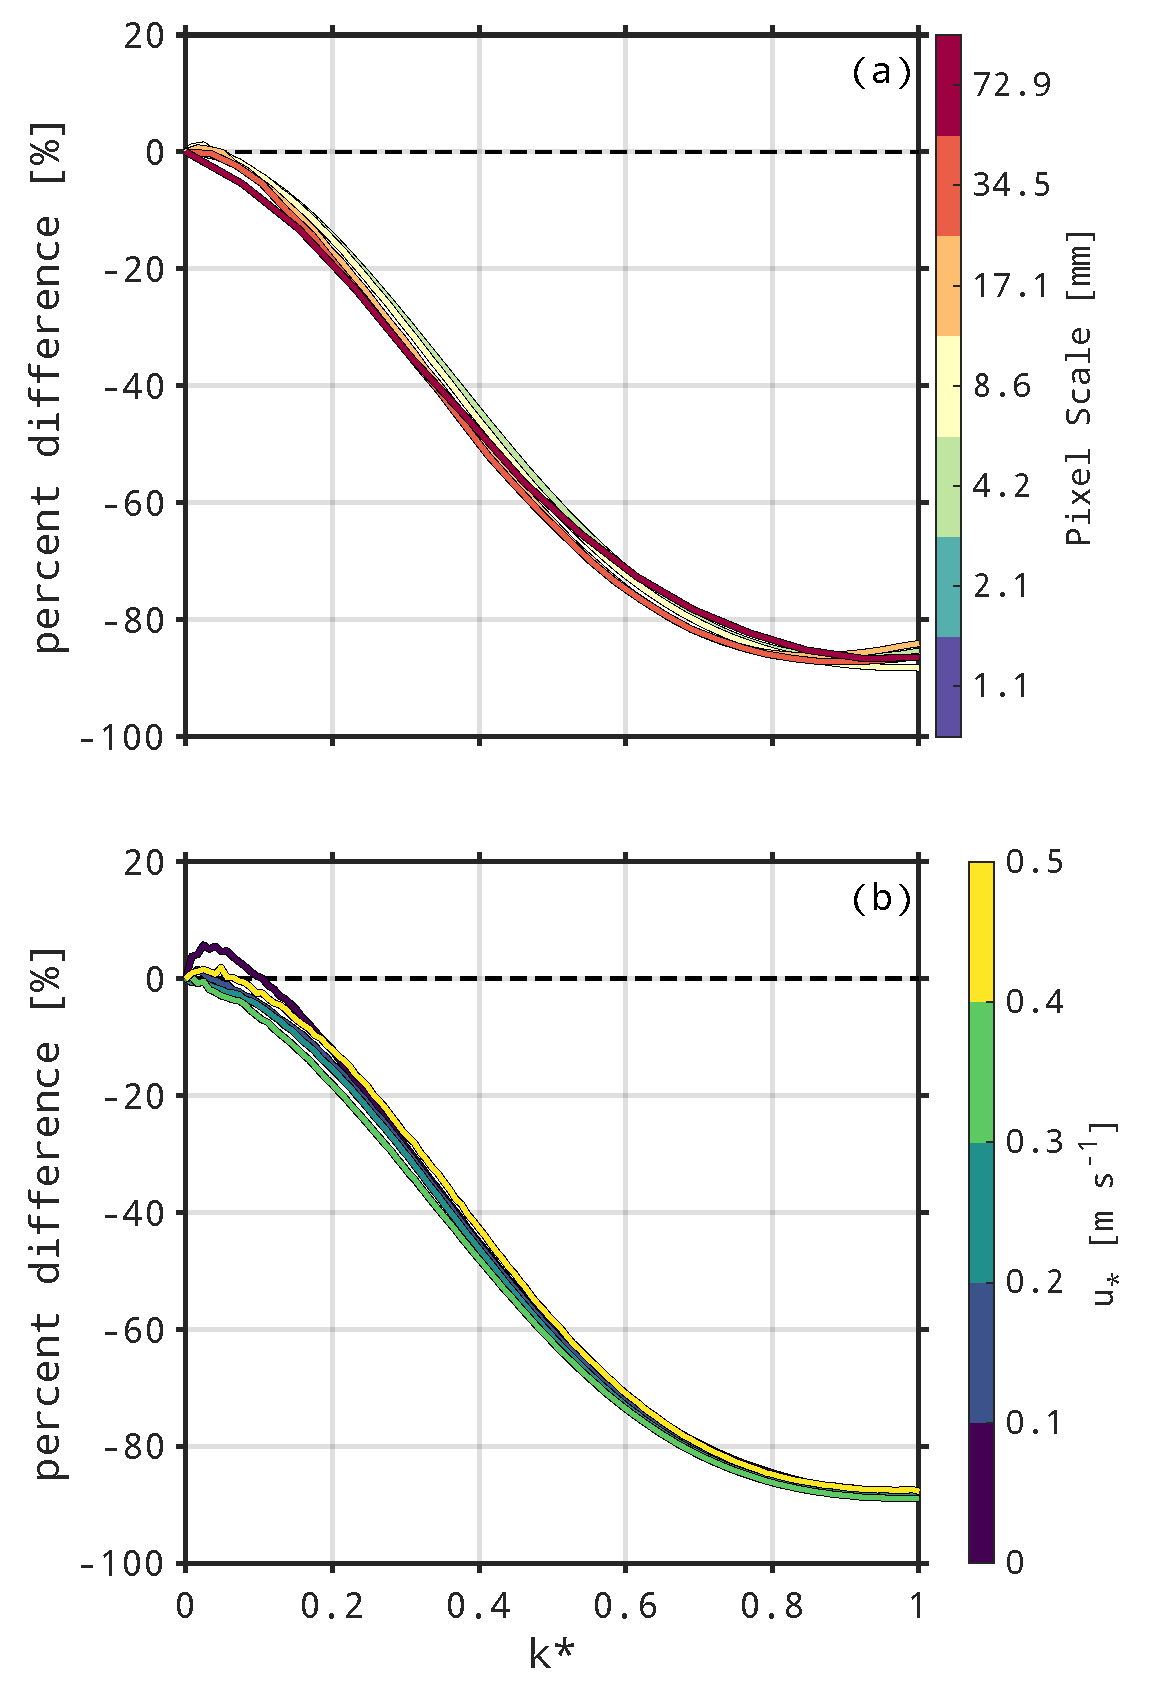
\includegraphics[width=0.5\textwidth]{_figures/block_averaged_ASIT_spectra_normalized.pdf}
% \vspace{-40pt}
% \caption{Percent difference between slope spectra computed from the full-resolution fields and those computed from the block-averaged fields. Panel (a) shows the average over all wind speeds, with color representing block-averaging size. Panel (b) shows the difference from all runs spatially averaged at 8.6 mm $\times$ 8.6 mm blocksize, averaged into five bins in air-side friction velocity. Wavenumber is normalized according to equation \ref{eq:k_star_definition}.}
% \label{fig:block_averaged_ASIT_spectra_normalized}
% \end{figure}

% \newpage

% \begin{figure*}[!hb]
% \centering
% 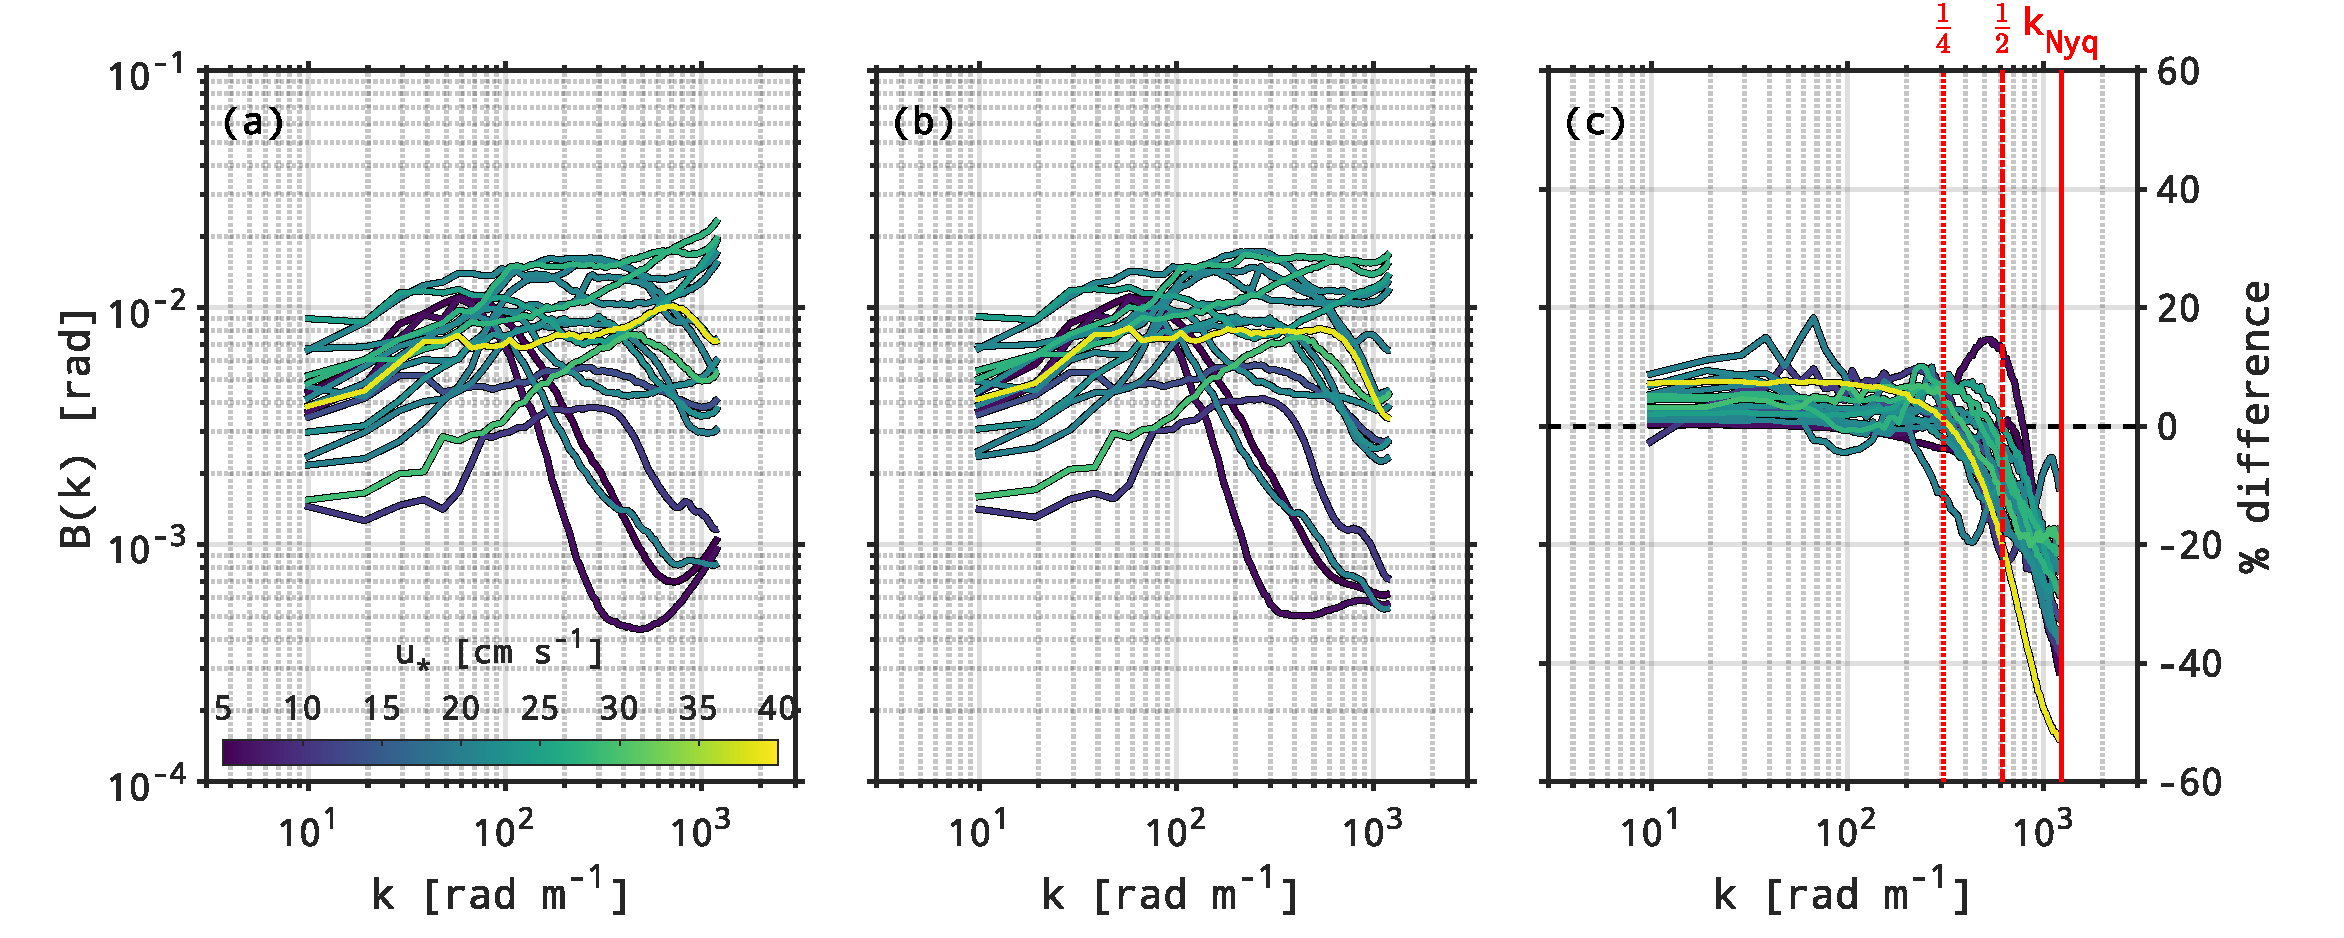
\includegraphics[width=\textwidth]{_figures/RaDyO2008_DoFP_sim_spectra_ratio.pdf}
% \caption{(a) Saturation spectra produced from wave slope fields obtained during RaDyO 2008 \cite{Zappa2012,Laxague2018b}. (b) Same, with a simulated DoFP array and bilinear interpolation of intensities. (c) Percent difference between original and simulated DoFP spectra. Color indicates air-side friction velocity $u_*$.}
% \label{fig:RaDyO2008_DoFP_sim_spectra_ratio}
% \end{figure*}

% \newpage

% \subsection{Investigation of DoFP-specific effects}

% Our second area of inquiry centered around effects specific to the sparse polarization measurements made via DoFP array detectors. These effects were investigated through the intentional degradation of the polarization information obtained via a full-frame DoAm polarimeter in a way that imitates the measurement made via DoFP (as first presented in Figure \ref{fig:slope_intensity_degradation_flowchart}). Free surface angles and omnidirectional saturation spectra produced through imitation of the DoFP measurement process were compared to the corresponding products of the 2 $\times$ 2 block-averaged polarization intensity data. This intermediate step was performed in order to isolate any effects specific to DoFP polarimeters from those which might be due to the simple spatial averaging described in the previous section.

% Spectra produced from slopefields computed from the 2 $\times$ 2 block-averaged intensity fields are shown below in Figure \ref{fig:RaDyO2008_DoFP_sim_spectra_ratio}a, with those produced from the imitation DoFP measurement given in Figure \ref{fig:RaDyO2008_DoFP_sim_spectra_ratio}b. The percent difference between the two follows in Figure \ref{fig:RaDyO2008_DoFP_sim_spectra_ratio}c; a positive (negative) difference indicates that imitation DoFP spectral density is increased (decreased) relative to the reference spectral density. For all wind speed conditions, the DoFP imitation yields spectra with energy density that is reduced at high wavenumbers relative to the spectra computed from simple block-averaged intensity fields. This diminution is substantial: up to $\approx$50\% for scales near the reduced Nyquist wavenumber of $\approx$1200 rad m$^{-1}$. However, it is mostly isolated to the tail, with energy density for wavenumbers less than half the Nyquist ($\approx$600 rad m$^{-1}$) showing $\lessapprox$20\% reduction, and energy density for wavenumbers less than one quarter the Nyquist ($\approx$300 rad m$^{-1}$) essentially unchanged. The full resolution example spectrum computed from slope fields actually obtained via DoFP detector (the violet trace in Figure \ref{fig:block_averaged_ASIT_spectra}) shows a dramatic fall-off for $k>0.5k_{Nyq}$. Although no extreme resolution reference point exists for these data, the diminished energy at high wavenumbers could be the result of effects specific to DoFP sensing.

% As with our other investigations, it was important to test the sensitivity of any such effects to the spatial area over which the measurement occurred. To be specific, the spectral comparison shown in Figure \ref{fig:RaDyO2008_DoFP_sim_spectra_ratio} was performed at a single resolution: 1.3 mm px$^{-1}$ at full-scale. However, given the dependence of RMSE angle on block-averaging size as described in section \ref{sec:results_spatial_averaging}, it is reasonable to expect that errors associated with DoFP measurement might also increase in magnitude with expanding superpixel size. In Figure \ref{fig:RaDyO2008_DoFP_rmse_mss}a, we report the RMS difference in angle between observed slope fields computed from block-averaged intensity and those computed via imitation DoFP. We find that RMSE in angle increases with blocksize at all levels of wind forcing and for all levels of sub-block RMS slope. A trendline ($\propto$ blocksize$^{1/3}$) has been provided for reference, though we offer no geometric explanation for the particular functional form of that trend. The corresponding percent difference in mean square slope is given in Figure \ref{fig:RaDyO2008_DoFP_rmse_mss}b. For block sizes (i.e., our imitation \lq\lq superpixels") smaller than 10 mm, the use of DoFP-style observation and processing results in a difference in mean square slope of $\lessapprox$10\% relative to simple block-averaging of the polarized light intensity fields for all levels of wind forcing.

% Although RMSE tends to increase with blocksize for a given case/wind speed, it also appears to be the case that particular levels of angular error occur at corresponding values of sub-block RMS slope across \emph{all} wind speeds. In Figure \ref{fig:RaDyO2008_DoFP_rmse_mss}a, one can see a similar level of error ($\approx$2.5\%) for 50 mm blocksize at low wind as for 5 mm blocksize at high wind-- with both cases having sub-block RMS slope of $\approx$0.05. Similar patterns can be seen for increasing levels of sub-block RMS slope. The modeled subpixel RMS slope curves shown in Figure \ref{fig:subpixel_RMS_slope} of Appendix \ref{sec:appendix_subpixel_rms_slope} provide a bit more context: (1) for a given level of wind forcing, increasing the blocksize (decreasing $k_{cut}$) elevates the subpixel RMS slope; (2) a given level of subpixel RMS slope at almost every wind speed, albeit at different spatial scales.

% The low cost, broad commercial availability, and high fidelity of modern DoFP detectors have resulted in rapidly expanding use of the technology in recent years. Therefore, the present work is not intended to serve as a comprehensive overview of all challenges or opportunities associated with DoFP (or polarimetry in general). However, there is an additional wrinkle which bears mentioning before we continue: the problem of light rays encountering a polarizing filter oblique to the orientation of the microgrid. This effect becomes relevant when rays are not collimated before interaction with the focal plane array (as is the case with DoFP detectors) and has been shown to produce an aberration which varies with distance from the detector center \cite{pistellato_geometric_2024}. The DoFP observations we describe here were made with a 75 mm lens, allowing us to neglect the effects of light ray/microgrid obliquity on account of the very small FOV ($\pm$3$^{\circ}$ from frame center).

% The hybrid observation/modeling approach was essential for addressing the two concerns which motivated this work. The field observational datasets in our stewardship were not of sufficiently high spatial resolution ($dx\approx$0.1 mm) to yield a reference surface wave field with negligible subpixel slope variability. Indeed- the practical limitations imposed by detector sizes would require unsuitably small fields-of-view ($\approx$10 cm $\times$ 10 cm) in order to achieve such high resolution. By deploying a polarized light reflection model, we were able to achieve our desired sub-millimeter resolution while simultaneously capturing meter-length surface gravity waves. Furthermore, while our DoAm field dataset allowed for direct investigation of slope sensing effects associated with DoFP-type detectors, the small number of observational cases \cite{Zappa2012,Laxague2018b} prevented a systematic analysis of variation with wind speed. Therefore, a second field dataset (collected via DoFP detector at ASIT in Fall 2019) was included in order to expand our capabilities for investigating wave slope error metrics and changes to slope spectral density with varying block average size.

% When interpreting the results from multiple field datasets and numerical model output, it is useful to pose high-level questions that might synthesize the findings into clean take-home messages. One such question that follows the concerns raised at the outset and is particularly relevant to the practical application of PSS: Is there a particular \lq\lq cutoff" pixel scale at which one can no longer reliably obtain short wave information? The results of the simulation (Figure \ref{fig:simulated_and_ASIT_surface_angle_RMSE}) indicate that 1-2 mm resolution is the lowest resolution one might want for high-fidelity recovery of short-scale waves (RMSE $\theta$ and $\varphi$ $\leq$1$^{\circ}$). Complicating this picture is the fact that errors for pixel sizes in the millimeter-centimeter range appear depend strongly on the short wave spectrum (Figure \ref{fig:spectral_nudge_3panel}). As the short wave spectrum is not known \emph{a priori}, this introduces an indeterminate level of uncertainty-- not a comforting finding. The field observations used in support of this line of analysis also show that errors in $\theta$ and $\varphi$ tend to increase with block size-- albeit at a lower level and with a wider range of variation.

% Spatial averaging of polarized light intensity substantially reduces the spectral energy density at wavenumbers smaller than the Nyquist wavenumber (Figure \ref{fig:block_averaged_ASIT_spectra}). This effect is remarkably consistent across block-averaging size and wind forcing (Figures\ref{fig:block_averaged_ASIT_spectra_normalized}a-b, respectively). This unambiguous reduction in spectral density is disturbing information for those looking to use the entire spectral domain of their measurement. If one wishes to accurately describe the high-wavenumber (gravity-capillary to capillary) tail of the spectrum, it is likely prudent to target a resolution much higher than required in order to mitigate the negative side-effects associated with spatial averaging over regions with slope variability. However, we find only $\approx$5\% reduction in spectral energy density for surface waves with $k=0.1k_{Nyq}$. That is-- if one desires to reliably observe long surface gravity waves via PSS, their sensing system should be designed to have a ground sample distance that is 10 times smaller than wave scale of particular interest.

% \vspace{-10pt}

% \begin{figure}[!hb]
% \centering
% 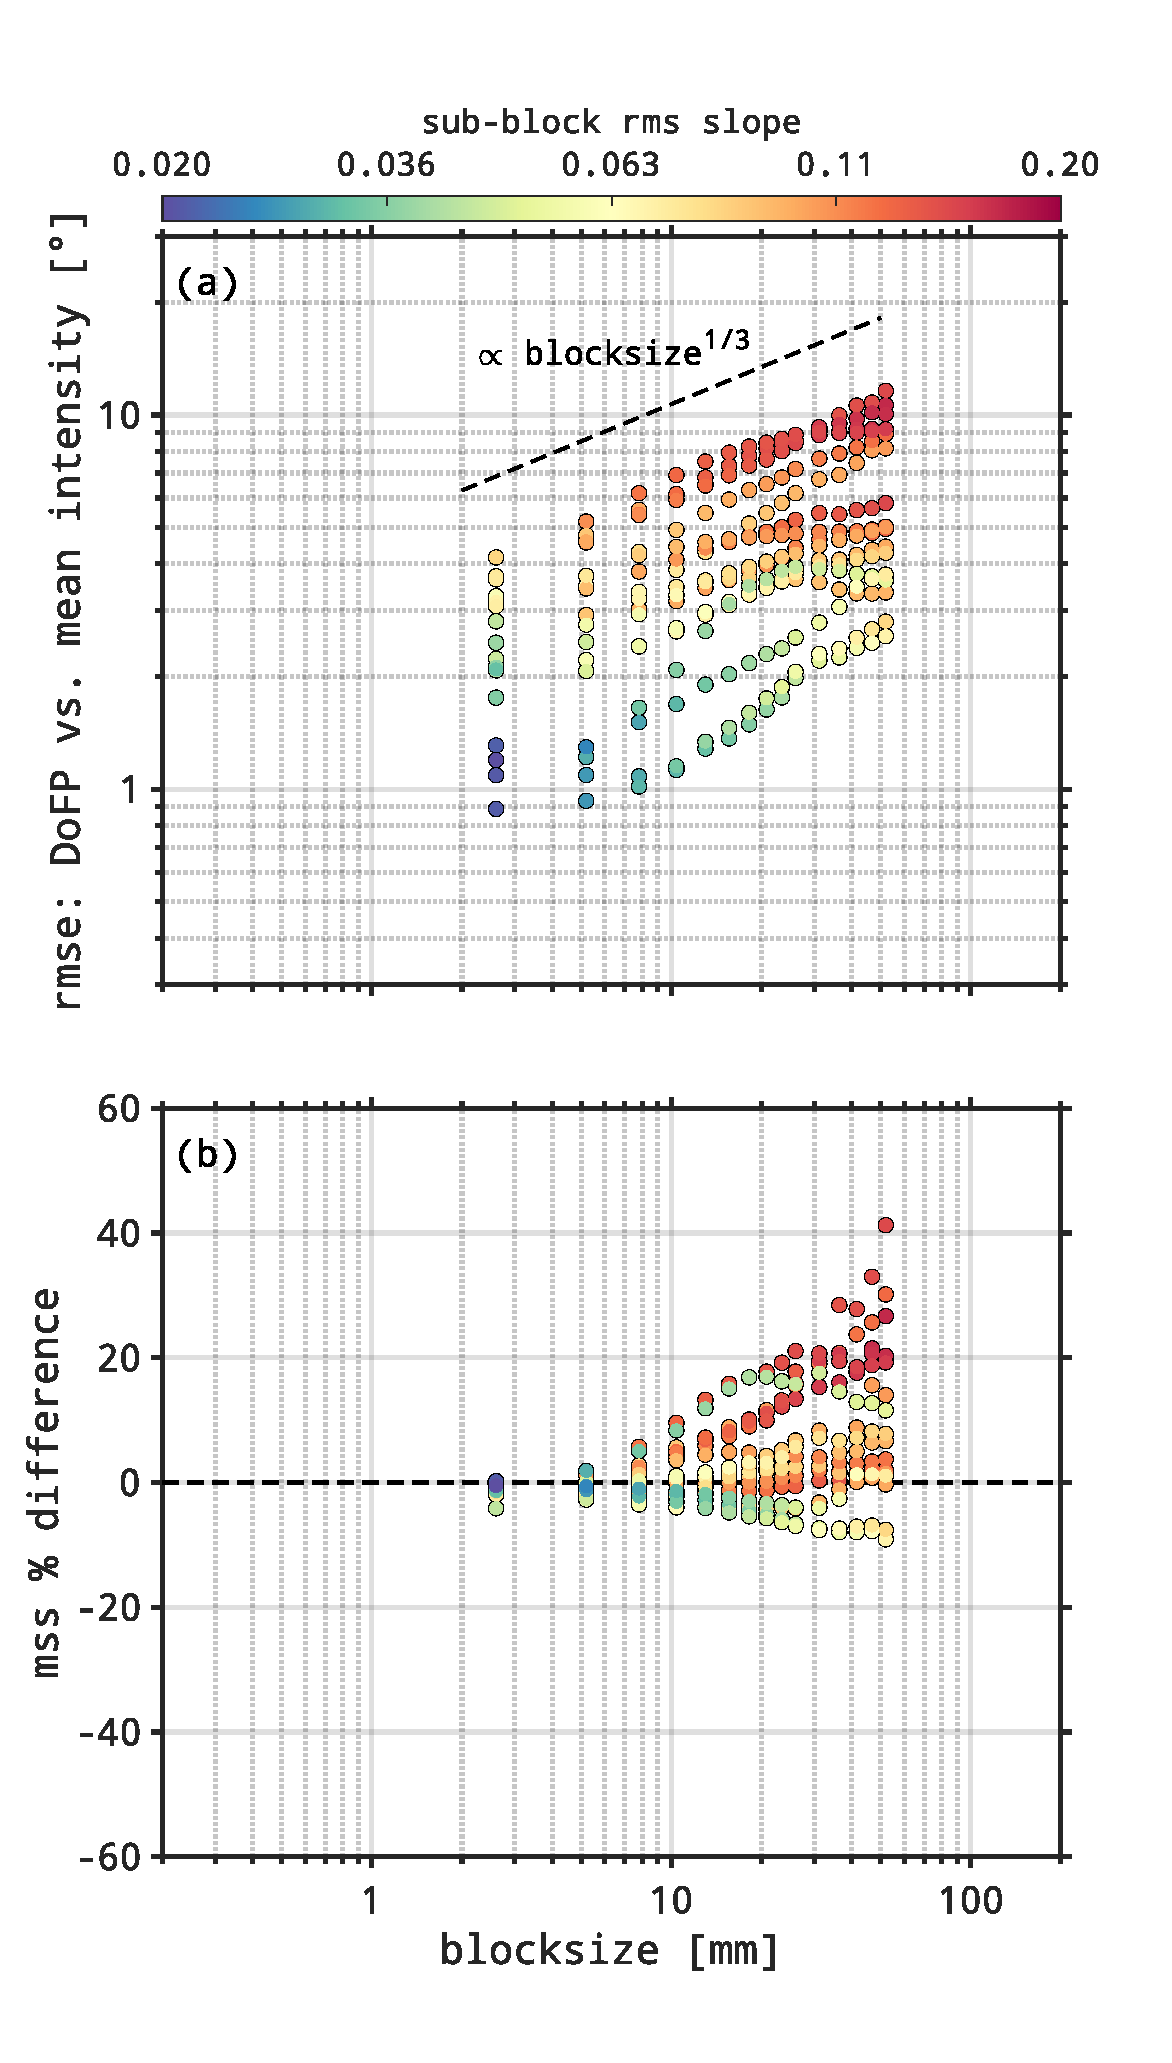
\includegraphics[width=0.5\textwidth]{_figures/RaDyO2008_DoFP_rmse_mss.pdf}
% \vspace{-30pt}
% \caption{Processing of DoAm polarimeter intensities to simulate effect of DoFP processing on surface slope at the level of individual points. (a) Total (along plus across-look) root-mean-square difference surface angle between (1) simulated DoFP processing and (2) block-averaged polarization intensities; (b) Ratio of mean square slope (mss) obtained from DoFP processing and mss obtained from slope fields computed from block-averaged polarization intensities. Both quantities are given in terms of block-averaging size and colored by the root-mean-square (rms) slope at scales smaller than the blocksize.}
% \label{fig:RaDyO2008_DoFP_rmse_mss}
% \end{figure}

% \newpage

% It is natural to extend this finding to the practical problem of quantifying long wave characteristics (e.g., significant wave height and gravity wave spectral density \cite{baxter_ocean_2012,johnson_ocean_2022}) via airborne polarimetry. Specifically, a 75-mm lens on a camera with the Sony Polarsens detector (3.45 $\mu$m pixel pitch) flown at an altitude of 100 m would have a field of view of approximately 10 m $\times$ 10 m, yielding strong response down to scales with $k=0.1k_{Nyq}\approx$32.1 rad m$^{-1}$ ($\approx$20 cm). Estimating performance at greater altitudes (and correspondingly greater pixel sizes, $\geq$10 cm) would require assumptions that the normalized spectral behavior shown in Figure \ref{fig:block_averaged_ASIT_spectra_normalized} is universal and not contingent upon sea state or observational parameters. Rather than make any such extrapolations, we reserve judgment until future observations can be made with a wider variety of lenses at a broader range of altitudes. There is an opportunity for low-flying UAV-based polarimetric slope sensing to validate and extend this spatial averaging analysis by acquiring surface slope fields at different altitudes for a given level of wind forcing.

% For DoFP-type detectors, increasing the effective pixel size appears to have two key negative outcomes relevant to the sensing of surface waves. The first is shown in Figure \ref{fig:RaDyO2008_DoFP_sim_spectra_ratio}, where we present evidence that the maximum wavenumber at which the wave spectrum may be reliably defined is not the Nyquist wavenumber $k_{Nyq}$, but 0.25-0.5 $\times$ $k_{Nyq}$. As we are computing the ratio between spectra produced via DoFP imitation and simple block-averaging, this reduction in spectral energy density exists \emph{in addition} to the effects shown in Figure \ref{fig:block_averaged_ASIT_spectra_normalized}. Taken at face value, these results indicate that up to half of the spectral domain obtained via DoFP array is negatively impacted by the mode of sensing. However, if one considers the array sizes (our DoAm: 768 $\times$ 576 pixels; the novel DoFP: 2464 $\times$ 2048 pixels), modern DoFP detectors are large enough to bear having their effective resolution halved while still making a fine-scale measurement.

% Furthermore-- this new effect may be at least partially due to image noise contamination of the smallest wave scales resolved via our DoAm detector. Evidence of this contamination comes in the form of upturned saturation spectra (i.e., \lq\lq flat" response of the slope spectra) at low wind (Figure \ref{fig:RaDyO2008_DoFP_sim_spectra_ratio}a). A recent \cite{laxague_suppression_2024} examination of a larger dataset of field observations made using the same camera revealed that the device was able to discern wave slopes as small as 0.01-0.02 (0.5-1$^{\circ}$). Whether the reduction in spectral density seen in Figure \ref{fig:RaDyO2008_DoFP_sim_spectra_ratio} constitutes attenuation of real wave energy or a benign smoothing through noise, it appears that little information is lost if one chooses to use a 4 $\times$ 4 demosaicking technique (e.g., the 12-pixel kernel offered by Ratliff \cite{ratliff_interpolation_2009}) rather than the 2 $\times$ 2 bilinear interpolation used here. The second negative outcome produced from our mimicry of DoFP-type sensing is shown in Figure \ref{fig:RaDyO2008_DoFP_rmse_mss}a: although error relative to simple block-averaging tends to increase with pixel (block) size, a stronger determinant of error is the wind speed (and often, therefore, the sub-block root-mean-square slope). There is a silver lining contained within Figure \ref{fig:RaDyO2008_DoFP_rmse_mss}b: even with moderate RMSE in surface angle (error in $\theta$ plus error in $\varphi$), estimates of total mean square slope are not substantially impacted until a single pixel reaches 1-2 cm (10-20\% error in mss).

\newpage



\vfill

\newpage

\section{Conclusion}

% At the outset of this paper, we identified two concerns associated with polarimetric slope sensing which arise from slope variability at scales below the measurement pixel size:\\
% \emph{C1: Spatial averaging of polarization state is not necessarily equivalent to spatial averaging of surface orientation.}\\
% \emph{C2: Polarization intensity measurements made by DoFP polarimeters are spatially sparse (non-collocated).}

% In order to test the degree to which these concerns impact the quality of measurements made through PSS, we pursued lines of analysis along three different trajectories:

% \begin{enumerate}[label=(\Alph*)]
%     \item Generation of a synthetic sea surface at sub-millimeter resolution, followed by implementation of a polarization-aware ray-tracing model to produce simulated fields of the Stokes parameters, yielding surface angles $\theta$ and $\varphi$.
%     \item Block-averaging of data collected via DoFP detector---either at the level of raw polarized light intensity or at the level of the computed slope field---for the purpose of simulating an increase in pixel spatial size.
%     \item Use of a high-resolution DoAm detector to obtain spatially collocated polarization information, modifying processing to mimic the sparse information of the DoFP detector.
% \end{enumerate}

% \noindent Our key findings are provided in list form below:

% \begin{itemize}
%     \item The results of our light reflection simulation indicate that millimeter-scale resolution is required to keep errors in surface angle $\lessapprox$1$^{\circ}$
%     \item The degree to which error varies with pixel size is itself dependent on the short wave (wavelength $\lambda\approx$ 1 cm) spectrum, an object which is unknown \textit{a priori}.
%     \item Increasing the spatial footprint of a pixel has a negative impact on the quality of the short wave measurement-- even at scales 4-8$\times$ larger than the pixel size.
%     \item However, wave scales greater than $\approx$20$\times$ the pixel size are well-resolved for pixels up to $\approx$75 mm in size, indicating that airborne PSS might be suitable for measuring longer surface gravity waves-- though future measurements are needed to test the upper limits of validity.
%     \item There is an additional penalty to resolution imposed by DoFP detectors which reduces the observed wave spectral energy density at high wavenumbers. We find that scales larger than 4$\times$ the pixel size are minimally affected.
%     \item If one simply wishes to obtain the total mean square slope (mss), DoFP detectors add no more than 10\% error for pixel sizes smaller than 1 cm.
%     \item A key driver of errors associated with larger pixel sizes appears to be the variability of slope at subpixel scales.
% \end{itemize}

% \noindent PSS is a powerful tool which enables measurement of surface waves at scales ranging from millimeters to decameters (and larger). We anticipate that our findings will help to guide the application of the technique, while the publicly-available processing framework will encourage its adoption. As the technique becomes more widely utilized, both our guidelines and processing framework will likely need to be refined. We believe that persistent (large sample size) and airborne (large FOV) PSS datasets are of particular value to this endeavor.

% \emph{Reference(s) for DoFP LWIR polarimeter?}

% \cite{caillault_multiresolution_2007}

% \cite{he_polarimetric_2018}

\newpage

\appendices

% \section{Subpixel RMS Slope in Terms of Cutoff Wavelength}
% \label{sec:appendix_subpixel_rms_slope}

% \begin{figure}[!ht]
% \centering
% 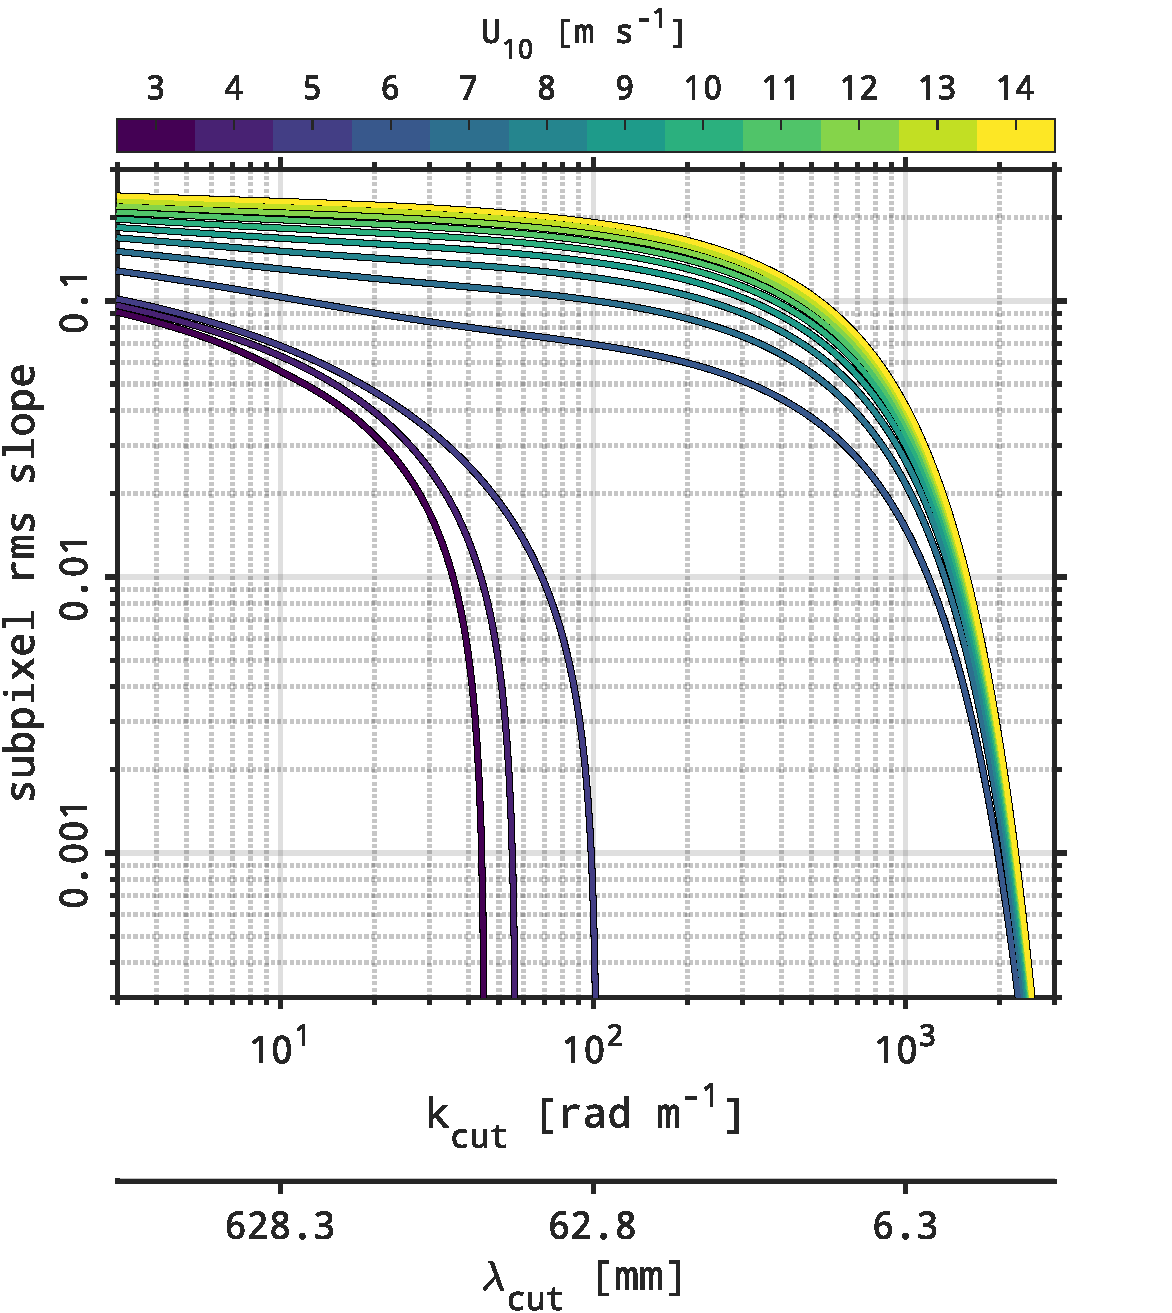
\includegraphics[width=0.5\textwidth]{_figures/subpixel_RMS_slope.pdf}
% \caption{Root-mean-square (RMS) wave slope associated with wave scales smaller than a cutoff wavelength $\lambda_{cut}=2\pi/k_{cut}$. Computed over a range of wind speeds using the model spectrum of Elfouhaily \emph{et al.} \cite{Elfouhaily1997}.}
% \label{fig:subpixel_RMS_slope}
% \end{figure}